\documentclass[12pt]{ucthesis}

\usepackage{etex}
\usepackage[morefloats=125]{morefloats}
\usepackage[hyphens]{url}
\usepackage{subfig}
\usepackage{graphicx}
\usepackage{tabularx}
\usepackage{amssymb}
\usepackage{amsmath}
\usepackage[letterpaper]{geometry}
\usepackage[overload]{textcase}
\usepackage{color}
\usepackage[nonumberlist,toc]{glossaries}
\usepackage{wrapfig}
\usepackage{longtable}
\usepackage{morefloats}
\usepackage{float}
\usepackage{listings}
\usepackage{makecell}
\usepackage{appendix}
\usepackage{cleveref}
\usepackage[]{algorithm2e}
\usepackage{titlesec}
\usepackage[breaklinks=true,hidelinks,pdfusetitle]{hyperref}
\usepackage{ifthen}
\usepackage[table]{xcolor}% http://ctan.org/pkg/xcolor

\def\CREATE{{\textsf{CREATE}}}

\makeindex
\makeglossaries

% Shrink the size of headers
\titleformat{\chapter}[display]
        {\normalfont\normalsize\centering}
        {\ifthenelse{\equal{\thechapter}{A}}{APPENDICES\\[4.3ex]}{}\chaptertitlename\ \thechapter}
        {0pt}{\normalsize\uppercase}
\titlespacing*{\chapter}{0pt}{-20pt}{4.3ex plus .2ex}


\titleformat*{\section}{\normalsize\bfseries}
\titleformat*{\subsection}{\small\bfseries}
\titleformat*{\subsubsection}{\small\bfseries}
\titleformat*{\paragraph}{\small\bfseries}
\titleformat*{\subparagraph}{\small\bfseries}

\bibliographystyle{abbrv}

\setlength{\parindent}{0.25in} \setlength{\parskip}{6pt}
\geometry{verbose,nohead,tmargin=1in,bmargin=1in,lmargin=1.5in,rmargin=1in}
\setcounter{tocdepth}{2}

% Different font in captions (single-spaced, bold) ------------
\newcommand{\captionfonts}{\small\bf\ssp}

\newcommand{\mycaption}[2]{\caption[#1 --- #2]{#1 --- #2}}

\makeatletter  % Allow the use of @ in command names
\long\def\@makecaption#1#2{%
  \vskip\abovecaptionskip
  \sbox\@tempboxa{{\captionfonts #1: #2}}%
  \ifdim \wd\@tempboxa >\hsize
    {\captionfonts #1: #2\par}
  \else
    \hbox to\hsize{\hfil\box\@tempboxa\hfil}%
  \fi
  \vskip\belowcaptionskip}
\makeatother   % Cancel the effect of \makeatletter
% ---------------------------------------

% Define Appendix refs
\crefname{app}{appendix}{appendices}
\Crefname{app}{Appendix}{Appendices}

\begin{document}

% Declarations for Front Matter
\title{CREATE: Clinical REcords Analysis Technology Ensemble}
\author{Skylar Eglowski}
\degreemonth{June} \degreeyear{2017} \degree{Master of Science}
\defensemonth{June} \defenseyear{2017}
\numberofmembers{2}
   \chair{Alexander Dekhtyar, Ph.D. \linebreak Professor of Computer Science}
   \othermemberA{Foaad Khosmood, Ph.D. \linebreak Professor of Computer Science}
   \othermemberB{Maria Pantoja, Ph.D. \linebreak Professor of Computer Science}
   \othermemberC{V.S. Subrahmanian, Ph.D. \linebreak Professor of Computer Science}
\field{Computer Science} \campus{San Luis Obispo}

\copyrightyears{seven}


\maketitle

\begin{frontmatter}

% Custom made for Cal Poly (by Mark Barry, modified by Andrew Tsui).
\copyrightpage

% Custom made for Cal Poly (by Andrew Tsui).
\committeemembershippage

\begin{abstract}
In this thesis, we describe an approach that won a psychiatric symptom severity prediction challenge. The challenge was to correctly predict the severity of psychiatric symptoms on a 4-point scale. Our winning submission uses a novel stacked machine learning architecture in which (i) a base data ingestion/cleaning step was followed by the (ii) derivation of a base set of features defined using text analytics, after which (iii) association rule learning was used in a novel way to generate new features, followed by a (iv) feature selection step to eliminate irrelevant features, followed by a (v) classifier training algorithm in which a total of 22 classifiers including new classifier variants of AdaBoost and RandomForest were trained on seven different data views, and (vi) finally an ensemble learning step, in which ensembles of best learners were used to improve on the accuracy of individual learners. All of this was tested via standard 10-fold cross-validation on training data provided by the N-GRID challenge organizers, of which the three best ensembles were selected for submission to N-GRID's blind testing. The best of our submitted solutions garnered an overall final score of 0.863 according to the organizer's measure. All 3 of our submissions placed within the top 10 out of the 65 total submissions. The challenge constituted Track 2 of the 2016 Centers of Excellence in Genomic Science (CEGS) Neuropsychiatric Genome-Scale and RDOC Individualized Domains (N-GRID) Shared Task in Clinical Natural Language Processing.  

\end{abstract}

\begin{acknowledgements}
\noindent
Thanks to:
\begin{itemize}
    \item Our team's work was supported by US Army Medcom/TATRC grant W81XWH-13-C-0030.
The CEGS N-GRID 2016 Shared Task in Clinical Natural Language Processing
 was sponsored in part by two NIH awards: NIH P50 MH106933 (PI: Isaac Kohane) and
NIH 4R13LM011411 (PI: Ozlem Uzuner).
    \item Andrew Guenther, for uploading this template
\end{itemize}

\end{acknowledgements}

\tableofcontents

\listoftables

\listoffigures

% Add CHAPTER into table of contents.
\addtocontents{toc}{%
   \noindent CHAPTER
}

\end{frontmatter}

\pagestyle{plain}

\renewcommand{\baselinestretch}{1.66}

\input{chapter-outline}

\chapter{Introduction}\label{sec:intro}

When a medical professional diagnoses a patient who is seeking help for mental health-related issues, there are two 
critical factors: correctness, and timeliness of the diagnosis. The correct diagnosis 
allows the clinical psychiatrist to devise and implement the appropriate
treatment. The timeliness of the correct diagnosis means that the appropriate treatment can start as soon as possible. 
Correctly assessing the severity of a patient's psychological symptoms poses a challenge with substantial negative consequences if estimated incorrectly.
If the severity of a patient's condition
is underestimated, the patient will not receive proper treatment, and the condition
may deteriorate; if the severity of the condition is overestimated, the
patient may be unnecessarily prescribed potentially harmful medications.

Therefore, initial psychiatric evaluations of patients play a crucial role in 
both the timeliness and the correctness of the diagnosis. Such evaluations 
often contain a plethora of information, including the patient's mental health history, the family's history of mental conditions, and a detailed report of the patient's 
present symptoms. Some of this data is naturally generated in a well-structured form: e.g. as a patient's answers to a series of self-assessment survey questions.
Other parts of the evaluations come as unstructured text: doctors' notes, patients' verbatim comments, and so on.

Track 2 of the CEGS N-GRID 2016 Shared Task in Clinical Natural Language Processing
challenged the participants to 
analyze the initial psychiatric evaluations of a group of patients for the purpose of predicting the severity of their symptoms. The challenge consisted of a two-month development stage with a labeled training set and a three-day window to submit labels for an unlabeled test set. The training set was composed of real world text and survey information with redacted names and dates. 
In this paper, we describe the methods used by our team to win this challenge, by leveraging known natural language processing (NLP) and machine learning methods into a
single pipeline we called \CREATE\ (Clinical REcords Analysis Technology Ensemble) shown in Figure~\ref{fig:arch}.

\begin{figure}[h!t]
	\centering
	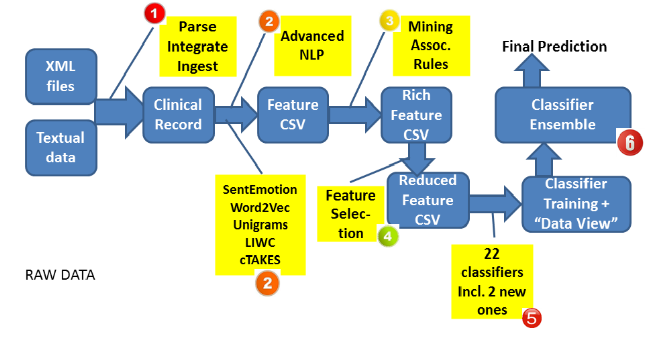
\includegraphics[width=0.95\textwidth]{figures/arch.png}
	\caption{Architecture of the \CREATE\ Framework}	
	\label{fig:arch}
\end{figure} 

The \CREATE\ framework is a machine-learning pipeline that includes several innovations. We start by taking the raw (noisy, cluttered) data provided to N-GRID challenge participants and use a data ingestion phase to ingest and clean it.
Second, we apply a host of sophisticated methods to extract a ``base'' set of  features for each clinical record from the ingested data. We expand this set of features
via a variety of methods, adding  8198 new features to the original 86. 
Third, we apply association rule mining to learn approximately 345,000 association rules
\cite{fpgrowth,c5}, and then trim them to a set of 628 predictive rules. Though association rules have been widely used in the literature for classification, we use them to generate 628 new features, one for each association rule.
Fourth, with the new total of $9284+628=9912$ features we engage a set of 
feature selection operations in order to eliminate useless features. 
Fifth, we train a total of 22 classifiers, each on seven different subsets
of features (data views). Of these, two are novel adaptations of existing Random Forest \cite{ho95,breiman01} and AdaBoost \cite{adaboost} classifiers. 
All of these classifiers build on top of the association rule classifiers developed earlier,
which is why we call them ``stackable'' in our framework. On our final step, 
we train different ensemble classifiers consisting of the subsets of best 
individual learners in order to improve the final accuracy of detection of
patient condition severity. In both the fifth and sixth steps, we do extensive k-fold cross validation and move forward from there to make our final predictions.

This is not the first time predictors have been stacked --- in the past, we developed stacked regressors for predicting airline market share and demand \cite{an2016map} as well as for predicting the number of hosts in a given enterprise that will be attacked by a given malware
\cite{kang2016ensemble}.

In addition, this is not the first time our team has worked with textual medical record classification. SentEmotion is a text-based classification engine that was developed in cooperation with psychologists. Leading surveys had identified a set of signals that a victim of depression might have: for example, isolation from others. SentEmotion signals were some of many features that we utilized in our final solution \cite{coptads}.

This paper is organized as follows. In Section \ref{sec:related} we discuss prior work in this area.  Section
\ref{sec:challenge} explains the details of Track 2 of the CEGS N-GRID 2016 Shared Task in Clinical Natural Language Processing (which we, for brevity, refer to as ``the N-GRID challenge"
throughout the rest of the paper) and provides an
overview of the data we have received from the challenge organizers.  
Section~\ref{sec:overview} provides an overview of \CREATE's six-step
approach to the N-GRID challenge.  Because Step 1 (ingestion and cleaning) is 
straightforward, albeit tedious, we do not describe it.
Section~\ref{sec:features} describes the features we used, while
Section~\ref{sec:assoc-rules} describes how we selected just 628 of 345,373 association rules  generated by an off-the-shelf association rule mining engine
called FP-Growth\cite{fpgrowth}, and by adapting Quinlan's C5 decision tree
induction algorithm \cite{c45,c5} for association rule mining. 
Section~\ref{sec:selection} shows how we determined 
which features (original and extended) were irrelevant.
Section~\ref{sec:ml} describes how  we engaged in an intensive classifier training and
hyperparameter optimization procedure on seven different data views of our dataset, 
which included the  adaptations of the well-known Random Forest and AdaBoost classifiers
for our purpose.  Finally, in Section \ref{sec:ensembles} we describe how we put together 
a variety of ensembles made from the best-performing individual learners, to 
improve the final prediction accuracy.
We conclude in Section~\ref{sec:conclusion}.

\chapter{Related Work}\label{sec:related}

Machine Learning another name for the task known as \textit{predictive modeling}: given a set of observations in the past, can you construct a procedure that can identify future observations correctly? There are several different types of classification problems, but the two that we will be focusing on are supervised and unsupervised classification. 

\section{Classification}

Classification is the act of associating an \textit{observation} with a pattern \cite{liu2007web}. Formally, an observation -- typically represented as a collection of text, audiovisual or numerical \textit{features} -- is assigned one or more labels. When presented with a new, unlabeled observation, the \textit{classifier} must \textit{infer} or \textit{predict} the most likely label to associate with the observation. For example, if a data scientist were tasked with classifying days as \textit{hot} or \textit{cold}, the number of customers at a local ice cream store could be used as a feature. In general, we'd expect the store to be more busy on hot days, rather than cold days. However, this is not a guarantee -- for example, a particularly large birthday party could form an outlier, or perhaps ice cream stores are just more popular on Fridays, even though Fridays are no more likely to be warmer than any other day.

An excellent classifier would be able to identify hot days from cold ones with high \textit{precision} as well as miss very few obviously hot days (known as \textit{recall}). In most tasks, data scientists must balance between both Recall and Precision. In some domains, recall is extremely important. For example, in the medical domain it is much preferred to have false positives while detecting cancer than it is to overlook a real threat at the risk of a patient's health.  On the other hand, some tasks prefer the opposite. A camera that detects if someone has run a red light would prefer to be precise rather than flag innocent drivers.

%% 
\subsection{Supervised Classification}

Supervised Classification is focused on identifying membership to one of a set of \textit{predetermined} patterns, typically called a \textit{label} \cite{liu2007web}. Supervised learning is called supervised because it is assigned a label by a human that is decided upon before the algorithm is trained. The \textit{training} step will be given each label, and the label must be trustworthy and consistent. Supervised Classification problems, therefore, tend to be somewhat expensive to collect data for. Every data point must be labeled and audited by a human, or even several in order to form a clear consensus.

In the following paragraphs, a brief description will be provided of a variety of the most common supervised machine learning techniques that we used as a part of \CREATE. 

\paragraph{Naive Bayes}

Naive Bayes is one of the simplest machine learning algorithms \cite{liu2007web}. During training, the classifier assumes that each feature is independent and marks two pieces of information: the distribution of labels in the training set, and the distribution of values for which a certain value of a certain feature is associated with label. During inference, it computes the probability of a new observation with its previously recorded values and predicts the most likely class.

\paragraph{Decision Trees}

Decision Trees are classifiers modeled after a flowchart. The final result of the classifier is a simple of yes/no questions, terminating with a final label at each of its terminal nodes -- called \textit{leaves}. Since computing the best possible decision tree is difficult (NP-complete), usually a set of heuristics are employed \cite{liu2007web}.

To construct the classifier, a recursive algorithm is employed. The base case is when the input computes only a single class, or if every single attribute has already been analyzed. In that case, the result is a leaf node of the majority class. Otherwise, each remaining attribute \footnote{for very large numbers of attributes, someones only a random sample is analyzed at each level} is analyzed to see which attribute splits the dataset into two ``pure'' disjoint sets best. The selected attribute is removed and phrased as a ``question'' in the final classifier, while each of the disjoint sets are re-evaluated recursively until each sub-problem is terminated with only leaf nodes.

\begin{algorithm}[ht]
\SetKwData{DecisionTree}{DecisionTree}
\SetKwData{ImpurityEvalA}{ImpurityEval1}
\SetKwData{ImpurityEvalB}{ImpurityEval2}
\SetKwData{ArgMax}{argmax}

\SetKwInOut{D}{D}
\SetKwInOut{A}{A}
\SetKwInOut{T}{T}

\D{True Labels}
\A{Features}
\T{Tree to recursively build (initially empty)}

\If{\textit{D} contains only one class}{
    \textit{make T a leaf node labeled with the majority class} \;
}
\ElseIf{\texit{A} is empty}{
    \textit{make T a leaf node labeled with the majority class} \;
}
\Else{
    \emph{(sometimes, only a random sample of attributes are tested)} \\

    $p_0 \gets $ \ImpurityEvalA{$D$} \;
    \For{$A_i$ in $A$}{
        $p_i \gets $ \ImpurityEvalB{$A_i, D$} \;
    }
    $g \gets $ \ArgMax{$p_1 \dots p_k$} \;
    \If{$p_0 - p_g < threshold$}{
        \textit{make T a leaf node labeled with the majority class}
    }
    \Else{
        $T_j \gets $ \textit{make T a decision node on $A_g$} \;
        \textit{partition \textit{D} into disjoint subsets for each value of $A_g$} \;
        \For{$D_j$ in partitions}{
            \DecisionTree{$D_j, A - A_g, T_j$} \;
        }
    }
}

\caption{Decision Tree construction \cite{liu2007web}}
\end{algorithm}

\paragraph{AdaBoost} \label{sec:adaboost}

AdaBoost is a methodology in which an \textit{ensemble} of weak learners are trained in succession; each learner specializing in correcting the errors the previous learner made. AdaBoost traditionally uses fast and weak learners such as Naive Boost or Decision Trees, as the initial weak learners only have to perform slightly better than random in order to eventually converge to a stronger classifier \cite{liu2007web}.

First, a base classifier is trained. Then, there is a \textit{boosting} step: this step computes all the training instances that were correctly or incorrectly identified. Those which were correctly identified are assigned a weaker level of importance for the successive classifier, while incorrectly classified observations are given a higher level of importance. Finally, the next classifier is trained with the re-weighted dataset \cite{adaboost}. 

The last two steps are repeated a predetermined number of times, or until a learner cannot improve on a previous learner. 

\paragraph{Random Forest}

Random Forests is an ensemble of Decision Trees that are trained on random subsamples of the training data \cite{breiman01}. Decision Trees suffer from a few disadvantages. First, for many problems decision trees tend to become very long and complex. This results in the tree overfitting the training data, and building patterns out of random noise; when you classify against out of sample data, it does not generalize very well.

However, you can generally eliminate this overfit without reducing performance by transforming the Decision Tree into a Random Forest. First, you must determine how many subtrees you would like to train.
Then, randomly subsample (with replacement) the data into that many subsets. Finally, construct a Decision Tree with each of those subsamples, with one small change: at each level of the Decision Tree subroutine, only sample a random subset of the features, rather than the entire feature set. This is to provide some entropy for the subtrees so that a handful of dominating features force almost every subtree to look the same. At inference, take the average of all the votes.

\begin{algorithm}
\SetKwData{DecisionTree}{DecisionTree}
\SetKwData{SubSample}{SubSample}

\SetKwInOut{D}{D}
\SetKwInOut{A}{A}
\SetKwInOut{B}{B}

\D{True Labels}
\A{Features}
\B{Number of subtrees to construct}

\For{$i$ in 0\dots$B$}{
    $D_i, A_i \gets $ \SubSample{i, D, A} \;
    $T_i \gets null$ \;
    \emph{only sample square-root features in each level of DT} \\
    \DecisionTree{$D_i$, $A_i$, $T_i$, \sqrt{A}} ; \\
    $Trees_i \gets T_i$ \;
}

\caption{Random Forest Construction \cite{scikit-learn}}
\end{algorithm}

\paragraph{Support Vector Machines}

Support Vector Machines attempt to identify how to bisect the feature space into two classes. Linear SVMs always bisect with a line in the form of $Ax + b = y$; though there are many \textit{kernels} that can be used to transform the feature space to solve more interesting problems. The observations closest to the bisecting plane are called \textit{support vectors}. In higher dimension problems, the composition of these vectors constructs a bisecting hyperplane. During inference, the label that is returned depends on whether the point is above or below the hyperplane.

\subsection{Unsupervised Classification}

Unsupervised Classification does not have labels, and instead attempts to assign certain patterns to groups, typically called \textit{clusters} \cite{celebi2015partitional}. Some algorithms expect hints in the form of the exact number or size of clusters, while others attempt to figure out it out on their own. Unsupervised classification is often used to provide insight for humans, especially for topic modeling \cite{celebi2015partitional}. Unsupervised classification can also be used as an automated way to learn compression and feature extraction methodologies, which is what we will focus on in the section \ref{sec:wordvectors}.  

\section{Text Representation and Word Vectors} \label{sec:wordvectors}

WordVectors \cite{word2vec} are currently the state-of-the-art method of representing text as features for supervised and unsupervised classification problems. However, the exact benefits of WordVectors are unclear without going over a brief history of simpler means of representation and textual feature extraction.

\subsection{Bag of Words}

\par{
The traditional method of text representation was a \textit{Bag of Words}. Bag of Words are unordered, sparse matrices where each column represents a unique term. As the English vocabulary $V$ is large and constantly changing, the first step of many Natural Language Processing tasks would be to scan over the corpus that you want to work with and build a list of each unique term. $V'$ is often smaller than $V$, but typos, proper names and slang all expand $V'$. For infinite datasets such as the Internet, one could utilize the \textit{Hashing Trick} \cite{weinberger2009feature} which runs each term into a hashing function that computes a random column index. This strategy has a few drawbacks such as colliding terms and having a $|V'|$ that is at least twice as large as your datasets predicted size, but no longer requires an additional pre-processing step.
}

%% Add citation for Singular Value Decomposition
\par{
Some classifiers, such as Naive Bayes \cite{rish2001empirical}, work with these very wide and sparse matrices very well. For classifiers that prefer small, dense matrices there are several strategies such as latent Dirichlet Allocation \cite{blei2003latent} and Singular Value Decomposition \cite{liu2007webi} that attempt to extract the most frequent and meaningful co-occurring terms and represent them as a single value. Moreover, additional information can be injected by extracting \textit{Parts of Speech} -- such as \textit{Noun} or \textit{Adjective} -- or constructing the \textit{lemma} of terms -- swimming $\rightarrow$ swim. 
}

\subsection{AutoEncoders}

\par{
AutoEncoders were originally designed as compression strategies for video and text and were a source of inspiration for WordVectors due to its ability to create graphical features in an unsupervised manner. Graphical data tends to be very high fidelity, and so transferring it over the Internet losslessly is expensive. In addition, small errors and loss of quality are not significant issues for videos that display dozens of frames per second.
}
%% Should it be "0...1" or are two periods standard?
\par{
Consider an grayscale image matrix $I$, that is \textsf{1000x1000} pixels. To simplify the problem, instead of a traditional RGB channel, each pixel is a float value in the range of 0\ldots1 indicating the grayscale of that pixel. Thus, the image contains 1 million floats if we were to represent it as a naive, dense matrix. Suppose our goal is to achieve 50\% compression. We would want to create two functions: $f_c$ and $f_d$. $f_c$ accepts $I$ and outputs a compressed version $C$ which is sent to the client, which $f_d$, then decodes and outputs $I'$. Our algorithm is trained to minimize the \textit{loss} which might be defined as the difference between $I$ and $I'$. Our black-box AutoEncoder would thus look something like this:
}

\begin{figure}[h]
\[f_c(I) => C \]
\[ f_d(C) => I' \]
\caption{S.t. $(I' - I)^2$ is minimized}
\end{figure}

%% Caption for AutoEncoder
\par{
Intuitively, there is a trade-off in $|C|$ and the loss. That is, smaller, more-compressed matrices will generally result in a higher loss $I'$. In a typical system, AutoEncoders are \textit{stacked}. That is, we might have three successive compression functions, each emitting a compressed matrix, followed by three successive decompression functions. The exact implementations of the AutoEncoder is beyond the scope of this discussion, but they generally rely on a Deep Neural Network \cite{tensorflow}.
}

\subsection{Word2Vec}

\par{
Mikolov's Word Vector model is one of the greatest recent developments in text classification \cite{word2vec}. Mikolov identified a few weaknesses of the Bag of Words model. First, constructing Bag of Word features requires two passes over the data \footnote{at least, not without using the Hashing Trick, which has its own drawbacks as discussed earlier}, which can be very costly when working with billions of documents. Second, if one could construct a model that captures all English literature with reasonable precision, then that model can be trained once and then used on nearly every English NLP problem. However, a "Universal English" Bag of Words model would be enormous and contain many unused words for most practical applications. The final and most significant flaw is how Bag of Words treats every word as equally distant from each other. This is intuitively imprecise. Words pairs such as \textit{\{\textit{lake}, \textit{swim}\}} or \textit{\{\textit{queen}, \textit{king}\}} are intuitively related compared to \textit{\{\textit{evil}, \textit{throttle}\}}.
}

%% Why aren't these paragraphs indented?
\par{
Word vectors solves this by constructing dense, continuous vectors with a limited number of dimensions such that similar words are closer than unrelated words. If vector space representations of \textit{queen} and \textit{king} were close, then we would have at least a partial success at solving the third problem. If our training model is capable of an online training that can handle billions of documents in a reasonable amuont of time, this would go a long way towards addressing the first two flaws.
}

\par{
Mikolov's initial paper described two methods: \textsf{skip-gram} and \textsf{continuous bag of words (cbow)}. \textsf{skip-gram} focuses on predicting a word's \textit{context} from the word itself, whereas \textsf{cbow} focuses on predicting a \textit{word} from its context. 
}

\par{
Consider $w_t$ which is defined as a word $w$ at location $t$. $w_t$'s context $C_t$ is defined by all words preceding or succeeding $w_t$ within a window of some parameter $n$. Now, we define a pair of functions $f$ and $g$ that are analogous to $f_c$ and $f_d$ in an AutoEncoder. $f$ accepts a sparse 1D vector where each column corresponds to a term in the vocabulary, just as it is in the Bag of Words model. $f$ will output a dense vector $V$ analogous to the compressed image $C$ in an AutoEncoder. In \textsf{skip-gram}, $f$'s input is $w_t$ and $g$'s output is $C_t'$, where the \textit{loss} is the difference between the predicted $C_t'$ and the actual $C_t$. In \textit{cbow}, $f$'s input is $C_t$ and $g$'s output is $w_t'$, where the \textit{loss} is the difference between the predicted $w_t'$ and the actual $w_t$. 
}


\begin{figure}[H]
\[ C_t: [w_{t-N}, \ldots, w_{t-2}, w_{t-1}, w_{t+1}, w_{t+2}, \ldots, w_{t+N}] \]
\caption{A Context $C_t$ is the Bag of Words representation of the \textit{window} centered at point $t$, with $w_t$ omitted}
\end{figure}


\begin{figure}[H]
\[ f(w_t) => V \]
\[ g(V) => C_t' \]
\caption{Skip-Gram: construct $f$ and $g$ such a word $w$ at location $t$ predicts its \textit{context} $C_t'$. The loss is the difference of $C_t'$ and its actual context $C_t$}
\end{figure}

\begin{figure}[H]
\[ f(C_t) => V \]
\[ g(V) => w_t' \]
\caption{CBOW: construct $f$ and $g$ such a context $C$ at location $t$ predicts \textit{word} $w_t'$. The loss is the difference of the predicted $w_t'$ and the actual word $w_t$}
\end{figure}

\par{
By itself, the \textit{skip-gram} and \textit{cbow} models do not seem to be useful. The key contribution of Word Vectors is understanding that unlike in an AutoEncoder where a human is consuming the final output $C'$, \textit{we can throw away $g$ and its output entirely!} Suppose we want to solve a second classification problem that has labels $L_t$. We can replace the original $g$ with a new $g'$ that accepts $V$ and predicts $L_t$! Thus, if we pre-compute a comprehensive look-up dictionary of words to $V$, we are able to greatly simplify the original dataset construction of multiple problems at the same time. 
}

\paragraph{Med2Vec} \label{sec:med2vec} Building on top of Mikolov's Skip-Gram model, Choi et al. sought to create a deep learning document embedding strategy \cite{med2vec}. They had two datasets of 3 and 5 million documents with a combined total almost 30,000 medical codes that acted as a natural clustering. \textsf{Med2Vec} is constructed in a similar method as \textsf{Skip-Gram Word2Vec}, but treats sequential visits from the same patient as if they were sequence of words in a sentence. Compared to \textsf{Skip-Gram Word2Vec} and \textsf{GloVe}, \textsf{Med2Vec} achieves lower, better normalized Mutual Information Gain scores on Medication and Procedure, implying that it builds embeddings that are better clustered for those tasks \cite{GloVe}. While \textsf{SVD} of document text performed better than \textsf{Med2Vec}, \textsf{SVD} was demonstrated to have far lower interpretability \cite{svd}. 

\section{Existing Medical Language Methodologies}

We limit discussion of existing methologodies to two categories:
work on analysis of clinical records in the medical domain, and emerging machine learning and NLP technologies.
In addition to these, our work on this project used a wide array of 
classification \cite{wu08} and association rule mining \cite{fpgrowth} techniques, and
traditional methods for text parsing and Parts-of-Speech (POS) tagging \cite{stanfordparser}. 
We used the Python \textsf{scikit-learn} \cite{scikit-learn} 
and \textsf{nltk} \cite{nltk} toolkits, the Stanford parser and Part of Speech Tagger \cite{stanfordparser}, and 
the Snowball stemmer for English\cite{snowball}. 

%% SKYLAR: EXPAND?
\paragraph{SentEmotion} 
Through its work on past projects \cite{dickerson14,kagan15,darpa} SentiMetrix has built an array of technology-based solutions, focusing on the near real-time analysis of large quantities of complex data in multiple languages. SentEmotion \cite{coptads-book,coptads} is a text-based classification engine developed jointly with psychologists that detects mental health disorders such as \textit{Depression}, \textit{Post-Traumatic Stress Disorder}, and \textit{Traumatic Brain Injury} from patient notes. Leading surveys had identified a set of signals that a victim of depression might have: for example, isolation from others. We built a classification engine on top of the Stanford Parser \cite{stanfordparser} to extract these signals, and then a second layer to extract both emotions -- anger or fear -- and symptoms -- insomnia or agoraphobia. The final layer generates a confidence value for each of the disorders that COPTADs is configured to recognize. 


\paragraph{cTAKES} Clinical Text Analysis and Knowledge Extraction System \cite{ctakes} by Apache is an open-source NLP system that extracts a variety of mental illness signals, physical symptoms, and medication from text.

%% TODO: cite apriori?
\paragraph{Classification using Association Rules} B. Liu developed a technique on which to do Classification Based On Association Rules \cite{cba}. Liu's main contributions is the notion of a \textit{coverage check} in which rules are sorted in order of their predictive power -- \textit{confidence} -- and then removes rules that are subsumed by a more powerful rule. At inference time, the first rule in which the antecedent is covered yields its corresponding class. Li et all improves upon this work by raising the minimum coverage of the \textit{coverage check} to 5 subsuming rules, as well as a stronger rule scoring using chi-$x^2$ tests \cite{cmar}. In addition, Li suggests storing rules in a trie so that inference can be performed quickly. 

\paragraph{Feature Selection using Association Rules} K. Rajeswari continued Liu's work to see if \textsf{Apriori} rule mining can be used select features with high significance, specifically in order to classify the risk of heart disease \cite{rajeswari}. First, the authors mined a set of rules with a small $k$ value. Then, they removed all features that did not appear in at least one rule. Next, they re-ran the \textsf{Apriori} but on a much larger $k$. Finally, when training the final classifier, they included only the features that were an antecedent in at least one rule. The higher $k$ value omits some useful association rules, but should take an order of magnitude less time to complete, due to the large reduction of $n$ candidate rules. The author conclude that this process reduces computation time on their dataset by two full orders of magnitude.

%%% TODO: expand this some more
\paragraph{Other Work} Abbe \cite{abbe} describes different styles of psychiatric NLP and suggests four domains: observational studies, analysis of patient's thoughts and journals, medical records, and published literature. The NGRID challenge falls into the third category, whereas SentEmotion mostly focused on the second. Pestian \cite{pestian} created an NLP pipeline that could identify whether or not a suicide note was genuine using decision-tree-based classification rules along with AdaBoost and outperformed domain experts by reducing Type II errors by 30\%.

\section{Ensemble Construction} Constructing ensembles was a key step in winning both the N-GRID competition as well as others, such as Kaggle. However, constructing ensemble rules by hand can be time-consuming or miss optimal solutions. Cortes et al. describes an online machine-learning algorithm called \textsf{ESPBoost} that accepts hundreds of potential ``experts" and the correct label \cite{espboost}. Similar to many other machine learning algorithms, \textsf{ESPBoost} uses coordinate descent to reduce a loss function -- in this case, Hamming -- to find a local minima without enumerating all possibilities \cite{coordinate-descent,hamming-loss}. \textsf{ESPBoost} has been empirically found to work best on large problems with a large number of experts.
 
\chapter{The Challenge}\label{sec:challenge}

The specification of Track 2 of the CEGS N-GRID 2016 Shared Task in Clinical Natural Language Processing  (also called the RDoC for Psychiatry Challenge) presented 
the goal of this particular track of the challenge as:
\begin{quote}
\textsl{``Determine symptom severity in a domain for a patient, based on information included in their initial psychiatric evaluation. The domain has been rated on an ordinal scale of 0-3. There is one judgment per document, and one document per patient."}\cite{N-GRID}
\end{quote}

Research Domain Criteria (RDoC) is a framework for facilitating the study of human behavior,
both normal and abnormal in various clinical domains. The RDoC provided the data,
originally collected by Partners Healthcare Inc. and the Neuropsychiatric Genome-Scale and RDoC
Individualized Domains (N-GRID) project at the Harvard Medical School \cite{N-GRID}.  The data
was released to the challenge participants under a strict set of Rules of Conduct and the Data Use Agreement.

As shown in Table \ref{tab:data1}, a total of 649 records were released,  broken into a training set of 433 files and 
a test set of 216 files with no ground truth --- the latter released two days before
the submissions were due. The initial release of the 433 patient records was broken into two categories: a suggested training set of 325 files, and 108 files
called \textsf{annotated\_by\_1}. Since the contest organizers discouraged us from using the records from the \textsf{annotated\_by\_1} set as training set data, we focused 
most of our efforts on the 325-record training set.

Each record, originally stored in a single XML file, represented the information from the
initial psychiatric consultation of a single patient performed by the N-GRID project. 
For each record in the training set the challenge organizers supplied the ground truth
about the severity of the patient's psychiatric condition, called \textsf{Valence}. Table \ref{tab:valence} shows the
scale on which the patients' conditions were evaluated.  The judgment contained in the \textsf{Valence}
field came from a clinical expert and was based solely on the symptoms and medical, social, 
mental health, and family history captured in the provided data.

\begin{table}
    \centering
    \begin{tabular}{|l|l|}
    \hline
    Total number of records released & 649  \\
    \hline
    Number of records in suggested training set    & 325  \\
    \hline
    Number of records in additional training set    & 108  \\
    \hline
    Number of records in test set   & 216 \\
    \hline
    \end{tabular}
    \caption{Overview of released data.}
    \label{tab:data1}
\end{table}


\begin{table}
\centering
    \begin{tabular}{|l|l|}
    \hline
    \textsf{Value} & \textsf{Meaning}\\
    \hline
    $0$  & \textsf{NONE}\\
    $1$  & \textsf{MILD}\\
    $2$  & \textsf{MODERATE}\\
    $3$  & \textsf{SEVERE}\\
    \hline
    \end{tabular}
    \caption{The scale of the target \textsf{Valence} variable in the N-GRID challenge training set data.}
    \label{tab:valence}
\end{table}

The  XML files provided by the challenge organizers contained both structured data, which documented
demographic information, mental health history, education, employment, financial status, family history of mental health, medical history, prescription and recreational drug use, and a few other categories of information; along with unstructured, free-form textual data, which documented self-reported symptoms and attending psychiatrists' notes on the patient and their condition. The data was in its raw, originally recorded form, and contained numerous typos, missing attributes, inconsistent use of abbreviations, and freeform text. The data was also anonymized.

Figure \ref{fig:sampleRecord} shows a \textit{notional (not real) record} created by us to illustrate the nature
of the data --- it contains no
information from the N-GRID dataset. However, this notional record
can give the reader an idea of the type of information that the teams had access to while working on the challenge
Actual records contained significantly more data.

\begin{figure}[t]
\begin{tabular}{|l|}
\hline
\texttt{RAW DATA}\\
\texttt{    Name: John Doe}\\
  \texttt{  Age: 42}\\
\texttt{    Sex: Male}\\
\\
    \texttt{Referred by Emergency Services}
\\    
\texttt{    Has difficulty remembering if he has taken prescription drugs.}\\ \texttt{Accidental overdose.}
\\    
\texttt{    Referral Notes: Patient exhibits short-term memory loss}\\
\texttt{Mixed alcohol with
    prescription. Stayed overnight.}\\
\texttt{Found bruises on shoulders - possibly from falling.}\\
\\   
  \texttt{  DEPRESSION: YES} \\
  \texttt{OCD: No}
\\
\texttt{    PANIC: Yes}
\\    
\texttt{    Prescriptions:}\\
    \texttt{ Advil (3 times a day)}\\
\\         
\texttt{    Formulation:}
\\
\texttt{    Patient has history of anxiety and bipolar.}\\
\\    
\texttt{    Recommendations:}
\\
\texttt{    Change medication to Alpazolam.}
\\
\texttt{    Require additional visit in 2 weeks.}
\\    
\hline
\end{tabular}
\caption{A synthetic record illustrating the type of clinical medical records data contained in the
dataset released for Track 2 of the N-GRID challenge.}
\label{fig:sampleRecord}
\end{figure}

Table \ref{tab:data2} contains a rough breakdown of the types of features found in the original data. Table \ref{tab:textdata} contains the list of features from the original data that were deemed by our team to be free-form text. In the original clinical files, features were informally grouped according to the idiosyncrasies of the RDoC system. The presented high-level feature groups are only given to help the reader understand the typical topics covered in a medical record.


%%% Moving the TEXT fields into a separate table.

\begin{table}
{\small
    \centering
    \begin{tabular}{|l|c|c|c|}
    \hline
    \textsf{Feature Type} & \textsf{\# features} & \textsf{Feature Type} & \textsf{\# of features}  \\
    \hline
    \textsf{All features} &       102    & &   \\ 
    \hline
    \textsf{Demographic information} & 3 & \textsf{Family History} & 4 \\
    \textsf{Harming Others Or Self} & 4 & \textsf{Symptom Denial} & 8 \\
    \textsf{Mental Health Symptoms} & 18 & \textsf{Owns Firearms} & 1 \\ 
    \textsf{Drug, Caffeine and Alcohol Use} & 5 & \textsf{Legal History} & 1 \\
    \textsf{Independence of Daily Activities} & 9 & \textsf{Appearance} & 14 \\
    \textsf{Marital Status and Abuse} & 3 & \textsf{Military History} & 2 \\
    \textsf{Employment and Finances} & 4 & \textsf{Mental Health} & 18 \\
    \textsf{If Underage, Legal Guardian} & 2 & \textsf{Physical Health} & 6 \\
    \hline

    \end{tabular}
    \caption{Breakdown of features in the original N-GRID 2016 challenge Track 2 dataset by category.}
    \label{tab:data2}
}
\end{table}
  
\begin{table}
    {\small
    \centering
    \begin{tabular}{|c|c|}  
    \hline
    \multicolumn{2}{|c|}{\textsf{Free-form Entries}} \\
    \hline
    \textsf{Childhood History} & \textsf{History of Present Illness and Precipitating Events}  \\
    \textsf{Previous Treatments} & \textsf{Prior Medication Side-effects} \\
    \textsf{Current Medication} & \textsf{Chief Complaint (Patient's Own Words)}  \\ %%% like how and where they grew up %%%
    \textsf{Interpersonal Concerns} & \textsf{Education}  \\
    \textsf{Family Living Situation} & \textsf{Protective Factors}  \\
    \textsf{Risk Factors} & \textsf{Actions Taken}  \\
    \textsf{Formulation} & \textsf{Level of Care} \\
    \hline
    \end{tabular}
    \caption{List of free-form text fields found in the original data for Track 2 of the N-GRID 2016 challenge.}
    \label{tab:textdata}
    }
\end{table}


The results of the challenge were evaluated using the a variant of the \textsf{Mean Absolute Error (MAE)} metric.  Given a vector $\mathbf{v} = (v_1,\ldots,v_n)$ of ground truth values and a prediction vector $\mathbf{p} = (p_1,\ldots, p_n)$, the \textsf{MAE} of the prediction is computed as  $$ MAE(\mathbf{p},\mathbf{v}) = \frac{1}{n}\sum_{i=1}^{n}| p_i - v_i|$$

\textsf{MAE} as described is frequently used in a variety of machine learning tests \cite{willmott2005advantages}. However, it has an unbounded maximal value, which can make it unintuitive to reason about. For this reason, the challenge organizes changed the formula such that the score was in the range of [0, 1], where 1 indicated a perfect score. The new \textsf{MA-MAE} (\textsf{Macro-Averaged Mean Absolute Error}) measure was computed
by splitting the set of records into four categories (one per ground truth \textsf{Valence} value), computing the \textsf{MAE} for each of the four subsets independently, and combining the computed \textsf{MAE}s into a weighted sum. The normalizing factors
for each of the component \textsf{MAE} values are the highest possible errors that
can be achieved for a data point with the given \textsf{Valence} value
($3$ for \textsf{Valence=0} and \textsf{Valence=3}, and $2$ for
\textsf{Valence =1} and \textsf{Valence = 2}).
To make the computed value correspond to the
\textit{higher is better} intuition, the computed weighted sum was subtracted from $1$.
The formula for computing the N-GRID Challenge version of \textsf{MAE} is:

\begin{figure}[H]
$$ MA\_MAE(\mathbf{p},\mathbf{v}) = 1 - 
    \frac{(\frac{MAE(\mathbf{P0}, \mathbf{V0})}{3} + 
     \frac{MAE(\mathbf{P1}, \mathbf{V1})}{2} + 
     \frac{MAE(\mathbf{P2}, \mathbf{V2})}{2} + 
     \frac{MAE(\mathbf{P3}, \mathbf{V3})}{3})}{4} $$
 \caption{Formula for computing Macro-Averaged Mean Average Error (MA-MAE)}
 \end{figure}


Every team participating in the challenge was allowed to submit up to three final guesses. Each guess was an XML file containing a single value which was the predicted valence for the specified clinical record from the provided \textit{test set}.

\chapter{Overview Of CREATE}\label{sec:overview}
Figure~\ref{fig:arch} describes the 6 parts of \CREATE.
We provide brief overviews of the individual components of \CREATE\  below.

%Because the data ingestion phase is relatively straightforward (but tedious), we do not describe it %below. The remaining 5 components are:

\begin{enumerate}
\item \textsf{Data Ingestion} - convert the XML data files provided to us into case $\times$ feature matrices that are readily consumed by machine learning pipelines. We limit our discussion of this step to what was presented in Section \ref{sec:challenge}, when we discussed the provided dataset.

 \item \textsf{Feature Extraction} - described in Section \ref{sec:features}.  We started our work on predicting the \textsf{Valence} variable by careful
extraction of existing features from the raw XML data provided to us by the  organizers.
After starting with the features present verbatim (i.e., as unique elements) in the released dataset (see Table \ref{tab:data2}) we defined several other features to generate a single overarching dataset.

 \item \textsf{Development of Association Rule-based Features} - described in Section~\ref{sec:assoc-rules}. In this stage, we extracted a set of 345,373 Class Association Rules from the above dataset and then eliminated redundant ones to generate a final count of 628. For each retained Class Association Rule we included a binary feature into our augmented dataset.
 
 \item \textsf{Feature Selection} - described in Section \ref{sec:selection}. We devised a set of tests to identify irrelevant features; a feature that failed all of the tests was eliminated.
 
 \item \textsf{Classifier Development \&\ Training} - described in Section \ref{sec:ml}. 
We devised seven different views of our data: each view containing a specific subset of the
full set of features. We put together a battery of 22 machine learning algorithms,
including two novel adaptations of Random Forests and AdaBoost. 
We trained the 22 classifiers on our seven data views and selected the best runs
for the ensemble learning step.

 \item \textsf{Ensemble Learning} - described in Section \ref{sec:ensembles}. On the
 last step, we evaluated ensembles of best-performing individual classifiers. 
 We used both simple majority/plurality ensemble schemes, as well as more complicated voting
techniques to see which, if any, provided the best solutions.
At the end, a number of \textit{simple} ensembles over subsets of our classifiers emerged with scores
that were clear improvements over the best  individual classifiers, and produced \textsf{MA-MAE} scores over 0.86.  From those, we selected three predictors that we submitted
to the N-GRID  challenge organizers.  
We are proud to report that one of our submissions had the
highest overall \textsf{MA-MAE} among the submitted solutions.
\end{enumerate}


\chapter{Feature Engineering}\label{sec:features}

To analyze the provided data, first we had to transform the original XML data into a tabular, textual format. Each XML file was structured so that it contained all the patient information in a single CDATA block, along with a single tag describing the Valence. Manual examination of several XML files revealed the underlying structure of the patient records (see the synthetic example in Figure \ref{fig:sampleRecord}).  
We have previously identified portions of the patient record that we elected
to represent as free-form text features (see Table \ref{tab:textdata}). 
These were primarily the restatements of  symptoms experienced
by the patients recorded from
their own words, plus notes and observations of the psychiatrists conducting the
evaluations of the patients.  Most other content from the XML files 
are represented as key-value pairs, with both keys and values relatively straightforward
to determine and extract. 

To transform this XML file into a pipeline-ingestable format, a serious of regular expressions were applied searching for text starting with a special \textit{key}. Pure textual data was assigned its own feature column, but would eventually be concatenated into one feature called \textsf{text\_ALL}. Ordinal numbers were simply used as is. Categorical values were handled on a case-by-case basis. Often, there was a limited number of potential values -- either text or numerical -- and we would map each categorical value to its own boolean feature, doing our best to map inconsistent abbreviation usage to the correct values. Missing data was represented with the value \textsf{Not a Number}. The final result of the extraction process, reduces the 102
features (identifiable in the XML files as individual prompts) to 86 features, which
we term the ``original" N-GRID dataset features.

The initial breakdown of features is described in Table \ref{tab:data2}.  As mentioned above, not every
 XML document had values for all of the extracted features; in fact, some features were
 present only in a handful of records, and other features were often omitted from records. Another data quality issue worth noting is the relative frequency of typos (which could have originated either from the process of digitization of the records, or from the initial medical records themselves). Regular expressions were used to reduce the amount of error in boolean and categorical entries. Some examples include catching different ways to say \textsf{No}: \textsf{N}, \textsf{Missing} or  \textsf{Not}. Other expressions simplified synonymous medical codes or shorthand in categorical features, such as \textsf{ld} for a \textsf{learning disability}. For free-form text, no typo detection or conjoined word detection was used. 
 
We have then proceeded to enhance the original N-GRID dataset with a wide range
of additional features. Below we discuss the nine different ways in which we augmented our feature set. Table \ref{tab:features} contains the summary of our feature
enhancement efforts.

\begin{table}[t]
 \centering
 \begin{tabular}{|l|l|c|}
    \hline
    \textsf{Approach}  & \textsf{Explanation} & $\#$  \\
    \hline
      \textsf{Original (Munged) Features}& Original clinical record entries & 102 \\
\hline
      \textsf{Cumulative Scores}& Aggregations of like features & 62 \\ 
      \textsf{Medications} & Individual medications taken by patients & 47 \\ %%% it was 374 unique names, 47 columns  
           
      \textsf{Association Rules} & ARs from features to \textsf{Valence}& 628\\
     
      \textsf{Unigrams} & Representations of textual data  & 8033 \\ 
      \textsf{Word2Vec vectors}& Representations of textual data & 300 \\
      \textsf{SentEmotion} & Sentiment and emotion extraction from text & 49 \\
      \textsf{cTAKES} & Medical symptom tagging & 658 \\
      \textsf{LIWC} & Topic detection and POS counts & 93 \\ 
      \textsf{Commonality of Patient} & A measure of how typical a patient is & 5 \\
      \hline
      \textsf{TOTAL} & & 9977\\
      \hline
 \end{tabular}
 \caption{A list of approaches to enhancing the feature set for the N-GRID Challenge (Track 2) dataset.}
 \label{tab:features}
\end{table}
 
 
 \section{Cumulative Scores}  Our initial investigation of the original 
 features extracted from the raw data unveiled groups of related features, typically
 with ``yes"/``no" values, where each individual feature was rarely set to ``yes" and no relationship with \textsf{Valence} appeared to exist. Moreover,
 the overall number of such features set to ``yes" in a single patient case history seemed to be in some relationship with \textsf{Valence}.  In such cases, we added a new feature: a
 \textsf{cumulative score} of ``yes" values in a group of features, to the dataset.
 
 For example, the original features contained a relatively rich arsenal of 
 substances that a patient could abuse or consume, from readily-available substances such as tobacco, caffeine, and alcohol to a wide range of recreational drugs. We identified all such features, and added a new feature
 \textsf{Cumulative\_Substance\_Use} which stored a count of substances which the patient
 admitted to using.  Similar cumulative count features were created for a few more 
 groups of variables: number of psychiatric review conditions deemed positive for the patient, number of ``abnormal" items from the mental status exam, number of activities
 the patient does not perform independently, and more.
 
 The reasoning behind adding such features to the dataset was straightforward: we saw features which appeared to carry important information, but which, due to relative lack of positive/abnormal/out-of-ordinary values, could not individually contribute to the learning of \textsf{Valence}. By creating cumulative count features, we represented the quantitative effects: case histories with more positive/abnormal responses in those feature columns received higher counts. This removed some of the sparsity of the dataset. 
 
 
%An additional category of cumulative features was a set of \textsf{typical score}
% features.  Many columns in the data were dominated by a single value (we called these 
% \textit{typical} values). While by itself, a typical value
% for a feature specifying that during the visit the patient was wearing socially acceptable
% clothing is not a very interesting observation, we recorded the percentage
% of features on patients' records that were marked with the ``typical" values
% for those features which may be of interest. As a result, we created a series of five 
%binary features: \textsf{typical51, typical67, typical80, typical90, typical95}.
%Each feature was set to 1 if the percentage of features set to ``typical'' values were 51\% ormore %for \textsf{typical51}, 67\% or more for \textsf{typical67} and so on.
 
 \section{Extracting Medications}  
 To capitalize on the possibility of using medications in predicting \textsf{Valence},
 we: (i)  manually created a list of 47 medications deemed relevant for
     patient conditions, complete with alternate spellings, brand names and abbreviations where applicable; (ii) developed a \textsf{Medication Extractor} which analyzed the input data and produced a list of all the medications listed within it; and (iii)
     created a dataset of medication mentions with 47 columns corresponding to each of the medications our \textsf{Medication Extractor} tool was tracking.     

  %% 
 \section{Emotion Features} SentiMetrix's SentEmotion is a web service,
 developed as part of the COPTADS project \cite{coptads-book,coptads} (see also Section \ref{sec:related}) that extracts the intensity of emotions such as anger, fear, depression, anxiety, stress, etc. from freeform text. In addition to labeling the overall sentiment of a text fragment
\cite{subrahmanian2008ava} and individual emotions expressed in the
 text (anger,  fear, depression, etc),  the system outputs a confidence value which expresses
 the level of confidence the system has in the presence of the emotion.
 We ran all textual information for each of the records through SentEmotion and
 added 49 new mental health-related features.
 
 %% STRIKEOUT
% While the richness of the data provided by the challenge organizers precluded us from
% relying on SentEmotion exclusively to analyze patient evaluations, we did use SentEmotion
% to collect the signals from the freeform text we extracted from patient records.
% Where SentEmotion features coincided with features that were already tagged in
% the patient record (for example, signs of depression), we did not use the SentEmotion signal.  However, we did use the final level of the results of SentEmotion
% classification process, and added each prediction as a separate feature to our dataset.
 %% TO SKYLAR: explain which exact features wound up making it into the dataset
 %%             and what "confidence" is.
 %% TO ALEX: okay well apparently this wasn't 100% true - we ended up keeping 49, not just 5 like i said originally
 %           i think this is something that i wanted to do and took it in my notes
 %           but VS had some push back or whatever. It's totally in the original dataset
 %           that said, most of the smx_signals didn't survive feature selection IIRC
 
 %% STRIKEOUT
 % For the purposes of the N-GRID Shared Task challenge, we used only the final level of classification as features: . Our rationale was that many of the signals were already annotated by an expert, such as the patient appearing fearful or crying. Rather than risk duplicating features, we fed the free-form text, such as patient history and personal description, as a single document into the COPTADs system. We then added each document's confidence value as a feature. 
\section{Simple Representations of Textual Information}
 At our initial examination of the provided data, we identified a number of features
 whose contents constituted free-form text. We considered using the free-form text from each of the features as a separate input into any text analysis procedures we were employing.
 However, in the end, we decided to concatenate the contents of all free-form features into a single free-form text feature, and conduct all text analysis on it. This resulted in the richest possible text being processed for each of our various patient records. 
 
We investigated a number of different ways to represent textual data in our dataset. The first and most straightforward approach we took was a part of the SentiMetrix Common Pipeline framework for data processing and data ingestion. The steps are as follows: 
 
 %%     \item Removal of dates and integers from the dataset to be placed into \textsf{SMXDATE} and \textsf{SMXNUM} features
 
 \begin{itemize}
     \item Replace dates with a special tag of \textsf{SMXDATE}
     \item Replace integers with a special tag of \textsf{SMXNUM}
     \item Stopword removal using the suggested english stopword lists in NLTK \cite{nltk} and Scikit-Learn \cite{scikit-learn}
     \item Stemming using the Snowball Stemmer \cite{snowball}
     
     \item Term-Frequency Inverse-Document Frequency \cite{ir-textbook,tf-idf} of unigram features for each surviving word stem/term
     
\end{itemize}

 
 \section{Word2Vec for Textual Information} \label{sec:word2vec-for-textual-info} Our second approach used
 \textsf{Word2Vec} 
 methodology \cite{word2vec} introduced
 recently by Google.
to represent each word found in each freeform text as a vector of 300 features.
We used Google's own collection of Word2Vec vectors trained on the Google News
corpus and provided by Google \footnote{https://code.google.com/p/word2vec/} . Despite N-GRID data containing many
specialized technical terms from the psychiatric domain, and proper names such as
names of medications, 96.8\% of tokenized text contained in the N-GRID training set
was also found in the Google's \textsf{Word2Vec} dataset with a coverage of 78.4\% of unique words. Examples of
words not covered are typos such as \textsf{``weopons"}, \textsf{``ibuprofin"} or \textsf{``bipolaar"}; conjoined words such as \textsf{"employment.He"}; dates such as \textsf{"8/17/86"}; and medical jargon such as an exact dosage for a patient.

To represent the text from individual patient records, we took the vector
representations of each term found in the free-form text in the patient's record,
and computed the mean vector. This is the Word2Vec 
equivalent of the traditional Bag of Words model, and acknowledged as a naive baseline to construct a
\textsf{ParagraphVector} by Mikolov and Le \cite{doc2vec}.  This procedure added 300 features to our dataset. We used gensim to load the binary Word2Vec word-to-vector file \cite{gensim}. 
 
 \section{cTAKES Features} As mentioned in Section \ref{sec:related}, \textsf{Apache cTAKES} is a framework for extracting a variety of information from medical records.
 \textsf{cTAKES} looks for terminology related to medical symptoms, mentions
 of medications, body parts, procedures, diseases, disorders, and a few other
 categories of information.  For each patient record, we ran the concatenated free-form text
 extracted from the record through \textsf{cTAKES} to collect these signals.
 

 \section{LIWC Features}
  \textsf{LIWC}, Linguistic Inquiry and Word Count  \cite{liwc}, is a linguistic computerized text analysis tool similar to SentEmotion. 
 \textsf{LIWC} produces 93 signals, which include various low-level Parts-of-Speech analysis such as the number/frequency of pronouns; 
 semantic features such as if the document has a positive or negative tone; and basic topic-analysis such as detecting if the document focuses on home, money, leisure, the past, or friends.
 We have run the free-form text extracted from each record, collected all
 \textsf{LIWC} features, and added them to our dataset.
 
 %%% TO ALEX: honest answer: we use it as a stop gap for PoS summarization since we haven't really done much PoS historically at SMX. In the future i'm going to push a bit stronger for PoS instead of just naive unigram stems. 
 %%% it also includes the `topics` such as `liwc_risk`, `liwc_focuspast`, `liwc_space`, `liwc_work`, `liwc_leisure`

 \section{Common Value Features}
\textsf{Common Value Features} are another form of a cumulative feature, but rather than summarizing logically related features, they summarizes features that individually have little explanatory power.
For example most individual observations of a variety of patient behaviors
were labeled with the code \textsf{"WNL"} which is interpreted as \textsf{"within normal limits"}.  In fact, \textit{most} patients had \textit{all} their observations
set to \textsf{"WNL"}, so a group of \textsf{"WNL"}-valued features
formed a very well-defined, \textit{but not very interesting} frequent itemset.
%For example, for our 47 medications, it is significantly more frequent for a user to 
%not be prescribed a random set of five medications than not. 
These very frequent, but essentially benign itemsets give rise to a large number of 
useless association rules during the rule generation process. Since an exhaustive
mining process on our dataset is extremely slow for any $k$ greater than 4, these \textsf{very frequent itemsets} tended both to consume
significant CPU resources while not producing any interesting results.

To reduce the size of our market baskets, we created the concept of a \textsf{typical value}. We set up five separate "commmonality" thresholds: 51\%, 62.5\%,
75\%, 87.5\%, and 90\%.  Given a number $t$ from the list above, and given
a feature from our feature set,
a specific value of the feature was called $t$-\textit{common} if more
than $t$ percent of all records in the training set contained this value.

\par{
We aggregated the notion of $t$-\textit{commonality} by introducing
five \textit{common value features} into the dataset: one per commonality
threshold. The common values feature for threshold $t$ was set to the total number of other features in the given record which contained $t$-\textit{typical} values. See the algorithm described in Algorithm ~\ref{alg:commonvaluealg} for more detail.
These new features allowed us to quickly see whether a specific patient evaluation record yielded rare, atypical, or unusual values for its features.
}


\begin{algorithm}[h] 
 \SetKwData{RowRank}{RowRank}
 \SetKwData{Array}{Array}
 \SetKwInOut{Output}{output}
 \SetKwInOut{F}{f}
 
 \F{matrix of feature values}
 \Output{5 new common value features}
 
 \BlankLine
 $num\_common\_values \gets$ \Array{5} \;
 $common\_values \gets$ \Array{\RowRank{$F$}, 5} \;
 \For{for each feature column $f$ in $F$}{
    \emph{$freq \gets$ compute a histogram for $f$} \;
    $most\_freq\_val \gets argmax(freq)$ \;
    \For{$ndx, t$ in enumerate([0.51, 0.625, 0.75, 0.875, 0.90])}{
        $f$ is common for threshold $t$ \;
        \If{$max(freq) \geq t$}{
            $num\_common\_values[ndx]$ += 1 \;
            for each record \;
            \For{$r$ in $f$}{
                \If{$r$ == $most\_freq\_val$}{
                    $common\_values[r, ndx]$ += 1
                }
            }
        }
    }
 }
 \emph{normalize output so it is in 0\ldots1} \\ 
 $common\_values$ /= $num\_common\_values$ \\
 \caption{How to compute our 5 Common Value Features}
 \label{alg:commonvaluealg}
\end{algorithm}

\chapter{Class Association Rules}\label{sec:assoc-rules} 
 
 We decided to see if we could discover
 some clear dependencies between the features present in,
 potentially small, subsets
 of patients, and the value of their \textsf{Valence}. To test this,
 we engaged in the process of mining our feature data 
 for Class Association Rules.
 
 We constructed a subset of binary and categorical features found in the data.
 These primarily included the original features, medication and cumulative
 features, and a small handful of features retreived from other sources.
 With these features, we concentrated on discovery of class association rules
 of the form:
 $$ F_1,F_2,\ldots, F_k\longrightarrow \mathsf{Valence},$$

\noindent where $F_1,\ldots, F_k$ are conditions on the binary/categorical features. Table \ref{tab:AR}
shows the parameters for our Class Association Rule search; we pruned away all rules that
did not satisfy them.

%%% ALEX: Do we want to talk about the improvements we made to the python-fp-growth implementation?
%%% i made a few tweaks to handle CARs much better (rather than generating all ARs and then eliminating all non-CARs)
%%% performance increase of 50%, which is significant because higher k's (k=4, k=5) took days to complete
%%% also dropped memory by a large constant factor because i used Numpy arrays to hold the values which have a lot less overhead than traditional Python lists and sets - and we would have hundreds of thousands of nodes 
%% DONE

We used an existing Python implementation \cite{python-fp-growth} of the \textsf{FP-Growth} \footnote{
Since the original Python implementation is not actively maintained, SentiMetrix has a private fork of the repository.
SentiMetrix's API tweaks allow the emission of only Class Association Rules, rather than all Association Rules,
 support for aggressive filtering of redundant rules while mining and utilizes Numpy arrays rather than Python lists for more compact memory allocation and faster cache coherence \cite{numpy}. The overall improvements result in a modest reduction of memory, and a 33\% reduction in run-time. In addition, considering only Class Association Rules reduces the problem size by multiple orders of magnitude. This is significant, because even with these improvements mining higher $k \in \{4, 5\}$ took days to complete. 
 } \cite{fpgrowth} 
algorithm to perform an exhaustive search for Class Association Rules with
$k \in \{1,2,3,4,5\}$.  For larger values of $k$ ($k = 6\ldots 9$) we used
$C5$ \cite{c5,c45}, which is non-exhaustive.

\begin{table}
    \centering
    \begin{tabular}{|l|c|}
    \hline
    \textsf{Parameter} & \textsf{Value} \\
    \hline
    Minimal Support  &  20 records\\ 
    Minimal Confidence & 0.6 \\
    Maximal Inverse Confidence & 0.4\\
    Maximal Negative Confidence& 0.4\\
    \hline
    \end{tabular}
    \caption{Pruning conditions for Association Rule mining process.}
    \label{tab:AR}
\end{table} 
 
 %% TO SKYLAR: insert a couple of sentences about chi-square pruning here.
 %%% i believe this was DONE yesterday
 %%% TODO: cite CMAR... also i suppose we should be using the author's name here?

%% TO SKYLAR: some of this might migrate to the next section. Think about it.
 
 
  The discovered rules went through a rigorous pruning procedure. In addition
  to pruning away all discovered Class Association Rules (CARs) that did not
  pass the minimum standards shown in Table \ref{tab:AR}, we also conducted
  a $\chi^2$ test of significance for each discovered CAR (see Section \ref{sec:selection}
  for a more detailed explanation of the $\chi^2$ tests conducted). All CARs
  that did not pass the $\chi^2$ test at the significance level of
  $p=0.05$ were also eliminated from consideration. Essentially, failing
  the $\chi^2$ test meant that there are significant reasons to believe that 
  the CAR is a by-product of individual frequencies of the features it contained,
  rather than an actual meaningful relationship between these features and
  the \textsf{Valence} variable.
  
Finally, we performed a \textit{Coverage Test} as proposed by Li et al \cite{cmar}. The purpose of the \textsf{Coverage Test} is to reduce the set of CARs to the ones that most accurately describe our data while avoiding excessive duplication. First, we sorted all of our generated CARs by confidence, support and $\chi^2$ score from best to worst. Starting with the first rule, all documents with features in the antecedent of the rule were marked. Then, we advanced onto the second round and marked all documents with features in the antecedent of that rule. The process was repeated until each input record was covered. After a single document has been marked five times, we removed it from future consideration. If a rule did not ``cover"" any considered documents, we discarded the rule. Once all documents have been marked five times, we discarded all remaining rules. For more information, see \ref{alg:coveragecheck}.
 
\begin{algorithm}[h]
\SetKwData{Covers}{covers}
\SetKwData{Rank}{Rank}
\SetKwData{Zip}{Zip}
\SetKwData{Array}{Array}
\SetKwInOut{rules}{rules}
\SetKwInOut{observations}{observations}
\SetKwInOut{Output}{output}
\SetKwInOut{k}{k}

\rules{Sorted set of candidate association rules (best to worst)}
\observations{Set of observations to cover}
\k{number of observations to cover an observation}
\Output{A set of covering association rules}
\BlankLine

$observation\_counts \gets$ \Array{\Rank{$observations$}} \;
\For{$rule$ in $rules$}{
    $keep \gets false$ \;
    \For{$observation, count$ in \Zip{$observations$, $observation\_counts$}}{
        \If{$count < k$ and \Covers{$rule, observation$}} {
            $keep \gets true$\;
            \emph{increment the corresponding $observation\_count$} \;
        }
    }
    \If{$keep$}{
        \emph{add our current $rule$ to $output$} \;
    }
}
\caption{A naive CAR coverage check algorithm as described in \cite{cmar}} \label{alg:coveragecheck}
\end{algorithm}
 
 
 Altogether, the pruning process reduced the total number of CARs extracted from the data from 345,373 to 628.
 \textit{For each extracted Class Association Rule, we added one binary feature to the dataset,
 which was set to 1 on records where the antecedent of the Association Rule applied} \footnote{The conclusion of the CAR was not considered, as that would result in leaking the label information during training, nor could these features be constructed on a hidden test set}. Some examples
 of the Association Rules we mined during this process are presented in Table \ref{tab:ARexamples}. The first two rules were found by the \textsf{FP-Growth}
 process, and the third by \textsf{C5}.
 
 \begin{table}
     \centering
     \begin{tabular}{|l|l|c|c|c|}
    \hline
    \textsf{Antecedent}& \textsf{Valence} & \textsf{Support}& \textsf{Confidence}&
    \textsf{Neg. Conf.}\\
    \hline
    \texttt{patient is an inpatient} and  &    &     &   & \\
    \texttt{currently undergoing}& \textsf{SEVERE} & 22 & 21/22 (95.45\%)& 18.25\%\\
    $\ \ \ \ \ $ \texttt{ addiction treatment} & & & & \\
    \hline
    \texttt{patient NOT taking Aplenzin} and &   & & & \\
    \texttt{has no history of drug abuse} and & \textsf{MODERATE} & 25 & 20/25 (80\%) & 22.06\%\\
    \texttt{suffers from OCD} & & & & \\
    \hline
    \texttt{patient is NOT inpatient} and  & & & & \\
    \texttt{does not drink alcohol} and  & & & & \\
    \texttt{is NOT taking Allernaze} and  & & & & \\
    \texttt{is NOT taking Levothroid} and  & & & & \\
    \texttt{is NOT taking Cultivate} and & \textsf{MILD} & 73 & 67/73 (92\%)& 38.37\%\\
    \texttt{is NOT taking Abilify} and  & & & & \\
    \texttt{does not suffer from OCD} and  & & & & \\
    \texttt{has no history of violence} and & & & & \\
    \texttt{suffers from depression} & & & & \\
    \hline
     \end{tabular}
     \caption{Examples of discovered Association Rules.}
     \label{tab:ARexamples}
 \end{table}
 
\chapter{Feature Selection}\label{sec:selection}

Because we now had thousands of features to consider, we developed a
feature selection procedure that subjected each feature in our dataset to a battery of tests. \textit{Features that failed
every single  test were eliminated from consideration}.  
The battery of tests is described in the following sections, followed by a brief analysis of the surviving features.

\section{Association Rule test} This decision procedure is a simple existence check: \textit{keep a feature if it
appears in the antecedent of at least one of the 628 Class Association Rules
in our dataset.}

\section{Statistical Tests}

We used 3 statistical tests to filter features. Each of our three methods works best with different feature types and captures different associations with a class labels.

\subsection{$\chi^2$ test for categorical features}
We ran a $\chi^2$ test \cite{chisquare} for each categorical feature against the
\textsf{Valence} variable.  This test checks whether there are sufficient
grounds to believe that a specific categorical feature is associated
with another categorical feature purely by coincidence.  

Suppose a feature is completely uncorrelated with a valence. This means
that the distribution of its categories will be very similar to that of 
the distribution of the ground truth labels. Now, suppose a \textbf{YES} value for a particular categorical feature always corresponds to a \textbf{MILD} valence. If we have sufficient number of \textbf{YES} observations, we can compute the likelihood that this happened purely by chance -- which would quickly become very low. We
 rejected any 
categorical feature whose $\chi^2$ test yielded a p-value higher than $0.05$.
The $\chi^2$ test was implemented by using \textsf{scipy}'s
\textsf{chisquare} function to compute the p-value of each categorical feature \cite{scipy}.


\subsection{ANOVA F-test for continuous features} 
ANOVA F-tests are used to test the significance of a regression model \cite{anova}.
While we used the $\chi^2$ test to test for potential significance of our 
categorical features, we used the multi-way ANOVA F-test for all numeric features.
For each feature tested, we separated the data into four subsets, based on the 
value of the target {Valence} attribute. We then randomly sampled from these four groups. We then tested the means and standard
deviations in each of the four subsets to see if they represented similar or
different distributions, and compared them across our multi-way samples to see if there is a statistical bias. Similarly to the $\chi^2$ test, we set rejected any numeric attribute whose ANOVA F-test
produced a p-value of more than $0.05$. We used
scikit-learn's \textsf{f\_classif} function to 
compute the multi-way ANOVA tests \cite{scikit-learn}. 

\subsection{Mutual Information Gain test (MIG)}

Mutual Information Gain is typically used in measuring the robustness of clustering methods.
In unsupervised problems, MIG  is measured by calculating \textbf{P(X, Y)} - the probability that two variables \textbf{X} and \textbf{Y} occur in the same cluster - compared to the probability \textbf{P(X) * P(Y)} of their occurring in the same cluster by random chance. If there is a clear dependence  %% or anti-dependence
between the two variables, then the probability of \textbf{P(X, Y)} will be higher %% or lower
than \textbf{P(X) * P(Y)}. Recent research shows that MIG provides an additional level of feature selection in the context of textual classification and clustering \cite{Xu07}. In the case of supervised feature selection, we compare the entropies and distributions of \textsf{Valence} vs. each feature
using $K$ Nearest Neighbors. At the time of the N-GRID Challenge, \textsf{scikit-learn} \cite{scikit-learn}
did not have a completed implementation of
\textsf{mutual\_info\_classif}, but it was in the process of being developed. We ported \textsf{scikit-learn}'s partial implementation into our system.

\section{Linear SVM Recursive Feature Elimination}
Our final test involved running \textsf{scikit-learn}'s version
of the Support Vector Machine (SVM) classifier with
a linear kernel \cite{cortes95} and observe whether the feature survived the
\textit{Recursive Feature Elimination} process implemented
within it. An advantage of using a linear SVM to find support vectors is that 
it provided our system with multivariate feature selection.
In addition, $\chi^2$ test and our Class Association Rules only worked on categorical features, 
while Mutual Information Gain requires a heuristic \cite{Xu07} to operate on continuous features.
The Linear SVM recursive feature elimination allowed us an additional test on
the continuous features in our dataset.

\section{Surviving Features}

Table \ref{tab:data3} contains the overview of the features that
survived this process: i.e., that passed successfully at least one of
the tests from the list above. We make a few observations here
about the final shape of the dataset. Only \textsf{LIWC} did
not contribute any features. All other means of enhancing
non-textual features provided meaningful contributions, 
with \textsf{cTakes}, original dataset, and, interestingly
enough, our cumulative scores accounting for the
majority of non-textual features.  All five \textsf{Common Value}
features also made it. Our manual work on documenting
medications resulted in 10 out of 47 medication
features kept. 

An unexpected outcome of 
this process was an essential depletion of directly word related
features from the dataset. Only 34 out of 300 Word2Vec dimensions were kept. For non-Word2Vec features, only a single unigram survived -- ``\textit{other}''. 
This implies that the categorical and yes/no responses have far more predictive power  than long form text.

\begin{table}
    \centering
    \begin{tabular}{|l|c|c|c|}
    \hline
    \textsf{Feature Category} & \textsf{\# Features} & \textsf{Feature Category} & \textsf{\# Features} \\
    \hline
    \textsf{TOTAL} & 788 & & \\
    \hline
    \textsf{Original} & 30 & \textsf{cTakes} & 40 \\
    \textsf{Cumulative scores} & 34 & \textsf{Common Value} & 5 \\
    \textsf{Medications} & 10 & \textsf{Word2Vec} & 34 \\
    \textsf{SentEmotion} & 6  & \textsf{CAR} & 628 \\
    \textsf{Unigrams} & 1 & & \\
     \hline
    \end{tabular}
    \caption{Description of the final set of features remaining in our
    operational dataset after the feature selection (pruning) step.}
    \label{tab:data3}
\end{table}



\chapter{Classifier Training and Adaptations}\label{sec:ml}

%% 1. List all classifiers we used (including their origin - scikit-learn and such

\begin{table}[t]
{\small
    \centering
    \begin{tabular}{|l|l|l|l|}
    \hline
    \textsf{No.}& \textsf{Abbreviation} & \textsf{Classifier} & \textsf{Source}\\
    \hline
    1 & \textsf{SVM-Ini}& \textsf{AdaBoost \cite{adaboost} \cite{scikit-learn}} & \textsf{SentiMetrix} \\
      & \textsf{AdaBoost} & \textsf{1 round Linear-SVM \cite{cortes95}},  49 rounds of NB  & \\
    2 & \textsf{RF-reg-clf} & \textsf{Train: Regression RF \cite{ho95}}; & \textsf{SentiMetrix} \\
      & & \textsf{inference: Classification RF} & \\
    3 &\textsf{MI SVR}&  \textsf{Mutual-Info \cite{ross14} Feature Boosted SVM \cite{cortes95}} & \textsf{SentiMetrix} \\
    4 & \textsf{CMAR} &  \textsf{Classifier on Multiple Assoc. Rules \cite{cmar}}& \textsf{SentiMetrix} \\
    5 & \textsf{CMAR SVM}& \textsf{CMAR-Boosted \cite{cmar} SVM \cite{cortes95}}& \textsf{SentiMetrix} \\
    6 & \textsf{CBA} & \textsf{Classification Based on Associations \cite{cba}}& \textsf{SentiMetrix} \\
    \hline
    7 & \textsf{MB NB} & \textsf{Multinomial/Bernoulli Na\"{i}ve Bayes \cite{scikit-learn}} & \textsf{scikit-learn} \\
    8 & \textsf{Lin-SVM}& \textsf{Linear Kernel SVM \cite{cortes95}} & \textsf{scikit-learn} \\
    9 & \textsf{RBF SVM}& \textsf{Radial Basis Function Kernel SVM \cite{scikit-learn}} & \textsf{scikit-learn} \\
    10 & \textsf{LogReg} & \textsf{Logistic Regression \cite{scikit-learn}} & \textsf{scikit-learn}\\
    11 & \textsf{RF} & \textsf{Random Forests \cite{ho95}} & \textsf{scikit-learn} \\
    12 &  \textsf{Adaboost NB}& \textsf{AdaBoosted NaiveBayes \cite{adaboost}}& \textsf{scikit-learn} \\
    13 &  \textsf{KNN} & \textsf{K-Nearest Neighbors \cite{scikit-learn}} & \textsf{scikit-learn} \\
    14 & \textsf{SGD} & \textsf{Stochastic Gradient Descent \cite{scikit-learn}}& \textsf{scikit-learn} \\
    15 & \textsf{BRBM} & \textsf{Bernoulli Restricted Boltzmann Machine \cite{scikit-learn}} & \textsf{scikit-learn}\\
    %followed by Random Forest/KNN/SVM/LogisticRegression} \\
    16 & \textsf{RF-reg} & \textsf{Regression version of Random Forest \cite{ho95}}& \textsf{scikit-learn}\\
    17 & \textsf{Lin-SVM-reg} & \textsf{Regression version of Lin-SVM \cite{cortes95}}& \textsf{scikit-learn}\\
    18 & \textsf{RBF SVM-reg} & \textsf{Regression version of RBF SVM \cite{cortes95}}& \textsf{scikit-learn}\\
    \hline
    19 & \textsf{DNN} & \textsf{Deep Neural Network \cite{tensorflow}}& \textsf{TensorFlow} \\
    20 & \textsf{Deep \& Wide} & \textsf{Deep-and-Wide classifier \cite{tensorflow}}& \textsf{TensorFlow} \\
    \hline
    21 & \textsf{XGBoost}& \textsf{XGBoost (scalable gradient boosting) \cite{xgboost}}& \textsf{XGBoost} \\
    22 & \textsf{C5} & \textsf{C5.0 Decision Tree Classifier \cite{c5}} & \textsf{RuleQuest} \\
    \hline
    \end{tabular}
    \caption{All the classifiers that were tried as part of the N-GRID Shared Task Challenge}
    \label{tab:Classifiers}
}
\end{table}

%% 2. discuss how we ran any of the classifiers (where this is not immediately clear

For our next step, we have constructed a battery of 22 different classifiers
to train on the dataset we built on previous steps. 
Table \ref{tab:Classifiers} lists the classifiers we
used on this project. 12 of the 22 classifiers came from \textsf{scikit-learn}.
Another five classifiers came from the internal SentiMetrix implementations
primarily developed prior to the N-GRID challenge, but modified where needed
to work with the data from this challenge.  Additionally, we used two 
neural network learners from Google's \textsf{TensorFlow}: their deep neural network
implementation; and their so called \textit{deep and wide} classifier, which
combines neural nets (deep learning) with Support Vector Machines (wide learning).
Finally, two extra classifiers --- \textsf{XGBoost}, the boosted gradient classifier
\cite{xgboost}, and Quinlan's implementation of
C5.0 decision tree classifier \footnote{Due to licensing restrictions, we did not integrate C5.0 into the Common Pipeline Framework} \cite{c5} --- were used as well.

Of the 22 classifiers we used two, the Random Forest Regression with Classification Inference (\textsf{RF-reg-clf} in Table \ref{tab:Classifiers}, and the SVM-initialized
Na\"{i}ve Bayes AdaBoost were novel adaptations of the well-known
Random Forest \cite{breiman01, ho95} and AdaBoost \cite{adaboost} machine learning
techniques. They are described below.

\section{Classifier Adaptations}\label{sec:newml}

Our two novel adaptations of existing classifiers are discussed below. 

\subsection{Random Forest Regression with Classification Inference (RF-reg-clf)}
Random Forest is a powerful yet forgiving algorithm that can perform a modest amount of feature selection due to its subsampling \cite{breiman01, ho95}. In \textsf{scikit-learn}, there are both regression and classification modes of Random Forest \cite{scikit-learn}. As Valence can be treated as both a class or an ordinal value, we tried both methods. Since regression provides additional insight for the classifier, it often had slightly higher scores. However, regression biases the kernel into averaging around the mean of all the labels. The result of this is \textsf{MILD} Valences might be moved to be slightly more \textsf{MODERATE} and vice-versa. When it comes to building the ensemble, this small amount of drift can result in large classification errors if it causes the ensemble's vote to cross a rounding threshold. Our adaptation was to train the Random Forest on the regression version of the problem. Then, during inference, round the inferred value to the nearest Valence. 

\subsection{SVM Initialized AdaBoost (SVM-Init-ada)}
The novel technique we used on this project is the initialization of AdaBoost learning
process with SVM (\textsf{SVM-Init-AdaBoost} classifier in our parlance). AdaBoost trains
a sequence of  estimators one after another \cite{adaboost}. After each iteration, the training set is be reweighed; documents that were just misclassified will have their weight increased, while documents that were just classified correctly will have their weight decreased. This forces the next classifier to correct the mistakes its predecessor made. While AdaBoost is traditionally done a fast and weaker classifier such as Naive Bayes, any kernel can be used. 

In other project, SentiMetrix has had success by introducing a single round of a slow and strong classifier as a seed for AdaBoost \cite{darpa}. As Support Vector Machines was one of our better classifiers and provides a meaningful decision function, it works well as the bootstrapping classifier and provides an anchor for the weak classifiers. We modified the AdaBoost process as follows:

\begin{enumerate}
    \item \textsf{Step 1:} Run Linear kernel SVM classifier on input data. 
    \item \textsf{Step 2:} Analyze kernel decision function to reweigh document weights
    \item \textsf{Step 3\ldots52:} Run Na\"{i}ve Bayes classification 49 times, reweighing document weights after every iteration, and checking for convergence. Reaching convergence before 49 iterations will terminate the process early
\end{enumerate}

On the input N-GRID challenge data, linear kernel SVM produced better
accuracy results than a single Na\"{i}ve Bayes run. This allowed our 
modification of AdaBoost to start with a sufficiently accurate bootstrap.
This additional accuracy gained on the first step has proven to be 
a core factor in the overall accuracy of this classifier, as one
of its runs wound up being the best individual classifier in our
battery.


\section{Data Views}

Each of or 22 classifiers 
was separately trained on nine different \textit{data views} described
in Table \ref{tab:dataviews}.  A data view is a collection of features
onto which the data is projected prior to being supplied to the classifier.
Different subsets of features were selected due to their distinct origins,
and the desire of our team to see if certain minimalistic sets of
features contain enough information for training the classifiers.

Two of the nine data views listed, 
\textsf{ANOVA-wordvector-34} (the 34 \textsf{Word2Vec} features that
passed our ANOVA significance tests) and \textsf{WordVector}
(all 300 \textsf{Word2Vec} features) yielded abysmal accuracy for
all classifiers, and were eliminated from further consideration.

\textit{Of the remaining seven data views} one, \textsf{Full}, represents 
the entire collection of features selected during
the process described in Section \ref{sec:selection}, five are its subsets,
and one, \textsf{TF-IDF} is the complete set of tf-idf vectors
representing the textual portion of each record. The subsets
of the \textsf{Full} data view were selected to represent different categories
of features (\textsf{CARs}, \textsf{Numeric}\footnote{The name
of this view is a bit of a misnomer, and is kept for historical reasons.
This view includes both numeric and categorical features that
were present in the original dataset, as well as constructed
using \textsf{cTAKES}, SentEmotion, and \textsf{LIWC} toolkits.}) as well
as the best features that passed a specific test: $\chi^2$, ANOVA or Multiple
Information Gain. We experimented briefly with top 100, 82 \footnote{82 was the fewest number of significant features found by all three statistical measures -- $chi^2$ in this case} and top 75 best features
for each of the tests, but settled on top 50, as this provided better accuracy.

As a result, at the end of the process we had a total of $22\times 7 = 154$
trained (classifier,data view) pairs to go through. As a final preprocessing step, we normalized the data view as appropriate for each classifier. For most classifiers, the normalization centered each feature and scaled it to have unit standard deviation using the interquartile range. For classifiers that cannot use negative numbers, such as Multinomial NB, we did the above normalization and then rescaled the data in the range of $[0, 1]$. This was accomplished with \textsf{scikit-learn}'s \textsf{RobustScaler} and \textsf{MinMaxScaler}, respectively \cite{scikit-learn}. 


\begin{table}[]
    \centering
    \begin{tabular}{|l|l|l|c|}
    \hline
    \textsf{No.} & \textsf{Label} & \textsf{Explanation} & \textsf{Size}\\
    \hline
        1 & \textsf{Full} & All features that passed filtering & 788 \\ 
        2 & \textsf{Numeric} & All numeric (and categorical) filtered & 125\\ 
        3 & \textsf{CARs} & All CAR features & 628 \\
        4 & \textsf{TF-IDF} & All tf-idf unigram features & 8033\\
        5 & \textsf{WordVector}& All \textsf{Word2Vec} features & 300\\
        6 & \textsf{Chi-square-best50}& 50 features with highest $\chi^2$ value & 50\\
        7 & \textsf{ANOVA-best50} & 50 features with highest ANOVA F-scores & 50 \\
        8 & \textsf{MIG-best50} & 50 features with best MIG values & 50 \\
        9 & \textsf{ANOVA-wordvector34}& \textsf{Word2Vec} features that passed ANOVA& 34\\
    \hline
    \end{tabular}
    \caption{Different data views used for classifier training.}
    \label{tab:dataviews}
\end{table}

%% 3. Describe our evaluation procedure (10-fold CrossValidation)
\section{Classifier Training and Evaluation}

For each classifier -- data view pair
we used 10-fold Cross Validation across the entire training set of 433 data points
from both the official training set and the additional \textsf{annotated\_by\_1}
set, using a seeded stratified method provided by \textsf{scikit-learn}. For evaluating the pipelines, we performed a 10-fold Train \& Predict using the best hyper-parameters from the previous step across the organizer-recommended 325 training files. These predictions were eventually fed into the Ensemble Creation procedures. 

Scikit-Learn provides some utilities for hyper-parameter selection \textsf{RandomizedSearchCV} and \textsf{GridSearchCV} which allow an engineer to specify a parameter grid which will be either randomly sampled or exhaustively searched, respectively. The sheer number of parametric combinations for some pipelines, such as Bernoulli RBM followed by a SVM, were forced to use RandomizedSearch but GridSearch is preferred otherwise \cite{scikit-learn}.

Towards the end of the competition, we occasionally switched to using a pipeline trained on the 325 records from the training set, and predict the \textsf{Valence} of the 108 \textsf{annotated\_by\_1} dataset to make sure that there was no significant over-fitting (in addition to our usage of 10-fold cross validation). For every classifier except \textsf{XGBoost}, scores on the 108 \textsf{annotated\_by\_1} files were lower than the the 325 record test set.

\begin{table}[]
    \centering
    \begin{tabular}{|l|l|l|l|l|}
    \hline
    \textsf{No.} & \textsf{Name} & \textsf{Algorithm} & \textsf{View} \\
    \hline
    1 & \textsf{MNB-CARs} & \textsf{MNB} & \textsf{CARs} \\
    2 & \textsf{RF-full} & \textsf{RF} & \textsf{Full} \\
    3 & \textsf{RF-reg-full} & \textsf{RF-reg} & \textsf{Full} \\
    4 & \textsf{RF-reg-clf-full} & \textsf{RF-reg-clf} & \textsf{Full} \\
    5 & \textsf{Lin-SVM-chi2-best} & \textsf{Lin-SVM} & \textsf{chi2-square-best50} \\
    6 & \textsf{Lin-SVM-anova-best} & \textsf{Lin-SVM} & \textsf{ANOVA-best50} \\
    7 & \textsf{RBF-SVR-mig-best} & \textsf{RBF-SVR} & \textsf{MIG-best50} \\
    8 & \textsf{SVM-Init-Ada-CARS} & \textsf{SVM-Init AdaBoost} & \textsf{Rules} \\
    9 & \textsf{D\&W-num} & \textsf{Deep \& Wide} & \textsf{Numeric} \\
    10 & \textsf{DNN-full} & \textsf{DNN} & \textsf{Full} \\
    \hline
    \end{tabular}
    \caption{Abbreviated names for classifiers for the next sections}
    \label{tab:Best6ClassifierNames}
    
\end{table}

{\renewcommand{\arraystretch}{0.75}%
\begin{table}[]
    \centering
    \begin{tabular}{|l|c|c|c|c|}
             \hline
   \cellcolor{gray!15} \textsf{RF-reg-full} & \textsf{Pred NONE} & \textsf{Pred MILD} & \textsf{Pred MOD.} & \textsf{Pred SEVERE} \\
   \hline
   \textsf{True NONE} & \cellcolor{gray!15} 13 & 28 & 4 & 0 \\
   \textsf{True MILD} & 3 & \cellcolor{gray!15} 94 & 33 & 0 \\
   \textsf{True MODERATE} & 0 & 16 & \cellcolor{gray!15} 60 & 6 \\
   \textsf{True SEVERE} & 0 & 4 & 49 & \cellcolor{gray!15} 15 \\
   \hline
   \cellcolor{gray!15} \textsf{Lin-SVM-chi2-best} & \textsf{Pred NONE} & \textsf{Pred MILD} & \textsf{Pred MOD.} & \textsf{Pred SEVERE} \\
   \hline
   \textsf{True NONE} & \cellcolor{gray!15} 28 & 13 & 4 & 0 \\
   \textsf{True MILD} & 11 & \cellcolor{gray!15} 103 & 13 & 3 \\
   \textsf{True MODERATE} & 1 & 18 & \cellcolor{gray!15} 41 & 22 \\
   \textsf{True SEVERE} & 1 & 2 & 21 & \cellcolor{gray!15} 44 \\
   \hline
   \cellcolor{gray!15} \textsf{RBF-SVR-mig-best} & \textsf{Pred NONE} & \textsf{Pred MILD} & \textsf{Pred MOD.} & \textsf{Pred SEVERE} \\
   \hline
   \textsf{True NONE} & \cellcolor{gray!15} 17 & 25 & 3 & 0 \\
   \textsf{True MILD} & 10 & \cellcolor{gray!15} 90 & 30 & 0 \\
   \textsf{True MODERATE} & 1 & 26 & \cellcolor{gray!15} 43 & 12 \\
   \textsf{True SEVERE} & 1 & 1 & 47 & \cellcolor{gray!15} 19 \\
   \hline
   \cellcolor{gray!15} \textsf{D\&W-num} & \textsf{Pred NONE} & \textsf{Pred MILD} & \textsf{Pred MOD.} & \textsf{Pred SEVERE} \\
   \hline
   \textsf{True NONE} & \cellcolor{gray!15} 27 & 17 & 1 & 0 \\
   \textsf{True MILD} & 13 & \cellcolor{gray!15} 84 & 25 & 8 \\
   \textsf{True MODERATE} & 3 & 17 & \cellcolor{gray!15} 41 & 21 \\
   \textsf{True SEVERE} & 1 & 4 & 20 & \cellcolor{gray!15} 43 \\
   \hline
   \cellcolor{gray!15} \textsf{SVM-Init-Ada-CARS} & \textsf{Pred NONE} & \textsf{Pred MILD} & \textsf{Pred MOD.} & \textsf{Pred SEVERE} \\
   \hline
   \textsf{True NONE} & \cellcolor{gray!15} 30 & 2 & 13 & 0 \\
   \textsf{True MILD} & 9 & \cellcolor{gray!15} 96 & 21 & 4 \\
   \textsf{True MODERATE} & 1 & 16 & \cellcolor{gray!15} 58 & 7 \\
   \textsf{True SEVERE} & 0 & 2 & 14 & \cellcolor{gray!15} 52 \\
   \hline
   \cellcolor{gray!15} \textsf{MNB-CARs} & \textsf{Pred NONE} & \textsf{Pred MILD} & \textsf{Pred MOD.} & \textsf{Pred SEVERE} \\
   \hline
   \textsf{True NONE} & \cellcolor{gray!15} 31 & 14 & 0 & 0 \\
   \textsf{True MILD} & 16 & \cellcolor{gray!15} 103 & 3 & 8 \\
   \textsf{True MODERATE} & 5 & 33 & \cellcolor{gray!15} 34 & 10 \\
   \textsf{True SEVERE} & 1 & 6 & 5 & \cellcolor{gray!15} 56 \\
    \hline
    \end{tabular}
    \caption{Individual Confusion Matrices on the 325 document training set for the 6 Classifiers in the Competition-Winning Ensemble.}
    \label{tab:BestEnsembleClassifiersConfusionMatrix}
\end{table}} \quad


\begin{table}[]
    \centering
    \begin{tabular}{|l|c|c|c|l|c|c|c|}
          \hline
   \cellcolor{gray!15} \textsf{RF-reg-full} & \textsf{Prec.} & \textsf{Recall} & \textsf{MAE} & \cellcolor{gray!15} \textsf{D\&W-num} & \textsf{Prec.} & \textsf{Recall} & \textsf{MAE} \\
   \hline
    \textsf{NONE} & \cellcolor{gray!15} 0.812 & 0.289 & 0.733 & \textsf{NONE} & 0.614 & 0.600 & \cellcolor{gray!15} 0.859 \\
    \textsf{MILD} & 0.662 & 0.723 & \cellcolor{gray!15} 0.824 & \textsf{MILD} & \cellcolor{gray!15} 0.689 & \cellcolor{gray!15} 0.646 & 0.793 \\
    \textsf{MODERATE} & 0.411 & \cellcolor{gray!15} 0.732 & 0.809 & \textsf{MODERATE} & 0.471 & 0.500 & 0.732 \\
    \textsf{SEVERE} & 0.714 & 0.221 & 0.738 & \textsf{SEVERE} & 0.597 & 0.632 & 0.848 \\
   \hline
   \cellcolor{gray!15} \textsf{Lin-SVM-chi2} & \textsf{Prec.} & \textsf{Recall} & \textsf{MAE} & \cellcolor{gray!15} \textsf{SVM-Init} & \textsf{Prec.} & \textsf{Recall} & \textsf{MAE} \\
   \hline
    \textsf{NONE} & 0.683 & 0.622 & 0.844 & \textsf{NONE} & 0.750 & 0.667 & 0.793 \\
    \textsf{MILD} & \cellcolor{gray!15} 0.757 &\cellcolor{gray!15}  0.792 & \cellcolor{gray!15} 0.885 & \textsf{MILD} & \cellcolor{gray!15} 0.828 & 0.738 & 0.854 \\
    \textsf{MODERATE} & 0.519 & 0.500 & 0.744 & \textsf{MODERATE} & 0.547 & 0.707 & 0.848 \\
    \textsf{SEVERE} & 0.638 & 0.647 & 0.863 & \textsf{SEVERE} & 0.825 & \cellcolor{gray!15} 0.765 & \cellcolor{gray!15} 0.912 \\
   \hline
   \cellcolor{gray!15} \textsf{RBF-SVR-mig} & \textsf{Prec.} & \textsf{Recall} & \textsf{MAE} & \cellcolor{gray!15} \textsf{MNB-CARs} & \textsf{Prec.} & \textsf{Recall} & \textsf{MAE} \\
   \hline
    \textsf{NONE} & 0.586 & 0.378 & 0.757 & \textsf{NONE} & 0.585 & 0.689 & 0.896 \\
    \textsf{MILD} & \cellcolor{gray!15} 0.634 & \cellcolor{gray!15} 0.692 & \cellcolor{gray!15} 0.787 & \textsf{MILD} & 0.660 & \cellcolor{gray!15} 0.792 & 0.866 \\
    \textsf{MODERATE} & 0.350 & 0.524 & 0.745 & \textsf{MODERATE} & \cellcolor{gray!15} 0.810 & 0.415 & 0.677 \\
    \textsf{SEVERE} & 0.613 & 0.279 & 0.739 & \textsf{SEVERE} & 0.757 & 0.824 & \cellcolor{gray!15} 0.902 \\
   \hline
    \end{tabular}
    \caption{Multi-class Precision, Recall and MAE on the 325 document training set for the 6 Classifiers in the Competition-Winning Ensemble. Per-class MAE is normalized with the assumption that all predictions are maximally incorrect for each class.}
    \label{tab:BestEnsembleClassifiersMetrics}
\end{table}

\begin{table}[]
\centering
    \begin{tabular}{|l|c|c|c|c|}
        \hline
        \textsf{ Classifier } & \textsf{ MA-MAE } & \textsf{ ROC-AUC } & \textsf{ $R^2$ } & \\
        \hline
      \cellcolor{gray!15} \textsf{ RF-reg-full } & 0.776 & 0.683 & \cellcolor{gray!15} 0.554 & \\
       \cellcolor{gray!15} \textsf{ Lin-SVM-chi2-best } & 0.834 & 0.765 & 0.521 & \\ 
       \cellcolor{gray!15} \textsf{ RBF-SVR-mig-best } & 0.757 & 0.657 & 0.476 & \\ 
       \cellcolor{gray!15} \textsf{ D\&W-num } & 0.808 & 0.721 & 0.394 & \\ 
       \cellcolor{gray!15} \textsf{ SVM-Init-Ada-CARS } & \cellcolor{gray!15} 0.851 & \cellcolor{gray!15} 0.811 & 0.515 & \\ 
       \cellcolor{gray!15} \textsf{ MNB-CARs } & 0.835 & 0.773 & 0.459 & \\
        \hline

    \textsf{ Classifier } & \textsf{ Precision } & \textsf{ Recall } & \textsf{ F1-Score } & \textsf{ Accuracy } \\ 
    \hline
    \cellcolor{gray!15} \textsf{ RF-reg-full } & 0.650 & 0.491 & 0.495 & 0.560 \\ 
   \cellcolor{gray!15} \textsf{ Lin-SVM-chi2-best } & 0.649 & 0.640 & 0.644 & 0.665 \\ 
   \cellcolor{gray!15} \textsf{ RBF-SVR-mig-best } & 0.546 & 0.468 & 0.481 & 0.520 \\ 
   \cellcolor{gray!15} \textsf{ D\&W-num } & 0.593 & 0.595 & 0.593 & 0.600 \\ 
   \cellcolor{gray!15} \textsf{ SVM-Init-Ada-CARS } & \cellcolor{gray!15} 0.738 & \cellcolor{gray!15} 0.719 & \cellcolor{gray!15} 0.724 & \cellcolor{gray!15} 0.726 \\ 
   \cellcolor{gray!15} \textsf{ MNB-CARs } & 0.703 & 0.680 & 0.673 & 0.689 \\
   \hline
    \end{tabular}
    \caption{Summary metrics on the 325 document training set for each of the 6 Classifiers in the Competition-Winning Ensemble. All applicable metrics are macro-averaged when necessary. Higher is better.}
    \label{tab:BestEnsembleClassifiersMAMetrics2}
\end{table}

Of the 154 total runs, we selected the 12 learners who scored above 0.60
to use in the next step: ensemble training \footnote{the exact threshold is coincidentally -- there was a large gap between 0.60 and a next-best cluster classifier+dataview combinations of scores around 0.54. Altogether, more than half of classifier+dataview combinations did only slightly better or equal to random}.  Of these 12 learners, 10 participated in the five \textit{best} ensembles (see Section \ref{sec:ensembles}.) These 10 are shown in Table \ref{tab:Best6ClassifierNames}
 which associates an abbreviated naming convention for each classfier+dataview.

For the sake of brevity, we limit the demonstration and discussion
of the results of the individual classifiers to the six
classifiers from Table \ref{tab:Best6ClassifierNames} which
constituted our top performing classification ensemble.
These classifiers are:
\begin{enumerate}
\item \textsf{RF-ref-full}: the Random Forest regression run on the \textsf{Full}
data view.
\item \textsf{Lin-SVM-chi2-best}: Linear kernel SVM classifier run
on the 50 best features selected by the  $\chi^2$ test.
\item \textsf{RBF-SVR-mig-best}: Radial basis function kernel SVM regressor run on
the top 50 best features selected by the mutual information gain test.
\item \textsf{D\&W-num}: the TensorFlow's Deep and Wide classifier run on
the numeric and categorical features.
\item \textsf{SVM-Init-Ada-CARs}: SVM-initialized Adaboost running on our CAR features.
\item \textsf{MNB-CARs}: Multinomial Na\"{i}ve Bayes running on our CAR features.

\end{enumerate}

Table \ref{tab:BestEnsembleClassifiersConfusionMatrix} contains the
confusion matrices for these six runs, Table \ref{tab:BestEnsembleClassifiersMetrics}
shows precision, recall and \textsf{MAE} for each class, while Table~ \ref{tab:BestEnsembleClassifiersMAMetrics2}
document the overall accuracy metrics: \textsf{MA-MAE}, \textsf{RoC-AUC}, precision, recall, f-score and accuracy.  We discuss the work of individual classifiers
below.

Our \textsf{RandomForest} regression run on the full data view (\textsf{RF-reg-full})
tended to over-predict \textsf{MILD} and \textsf{MODERATE} valences at the expense of
\textsf{NONE} and \textsf{SEVERE}, however, it contained excellent separation 
between the \textsf{NONE}/\textsf{MILD}, and \textsf{MODERATE}/\textsf{SEVERE} pairs
of valences, with only \textsf{MILD}$\Rightarrow$\textsf{MODERATE} false positives
being of concern.  While this run had the second lowest \textsf{MA-MAE} value out of our
six runs, it should be noted (see Section \ref{sec:ensembles}) that this is \textit{the only}
run that participated in all final ensembles. 

The linear kernel SVM classifier running on our top 50 $\chi^2$ features
(\textsf{Lin-SVM-chi2-best}) has the third highest \textsf{MA-MAE} and
has produced an excellent confusion matrix, with majority of \textsf{NONE}
and \textsf{SEVERE} conditions being classified correctly, and with very few
``costly" misses.

The SVM regressor with RBF kernel running on our top 50 Mutual Information Gain features
(\textsf{RBF-SVR-mig-best}) had the lowest performance of these six runs
(although was still among the better classifiers overall). It over-predicted
the \textsf{MODERATE} class, and had some trouble distinguishing \textsf{MODERATE}
and \textsf{MILD} valences. It also was very strict at predicting \textsf{NONE}
and \textsf{SEVERE} valences.

TensorFlow's  Deep and Wide  classifier, run on all our
numeric and categorical attributes, excluding CAR and \textsf{Word2Vec}
attributes (\textsf{D\&W-num}) had no significant distinctive features as compared to
other runs. It did the worst on properly capturing \textsf{MILD} valences
(\textsf{MILD} recall), and tended to admit more "big" mistakes
(misclassifications two or more classes apart) than some other methods. 
But it kept the overall number of misclassified cases reasonable,
and hence earned a \textsf{MA-MAE} in excess of 0.8.

Our overall best single run came from our own AdaBoost classifier
trained on a single round of SVM followed by 49 rounds of Na\"{i}ve
Bayes applied to the dataset consisting solely of \textsf{CAR} attributes
(\textsf{SVM-Init-Ada-CARs}, see Section \ref{sec:newml}). 
This classifier excelled almost everywhere, giving by
far the most accurate predictions of \textsf{SEVERE} valence and minimizing
false positives. The only ``weak spot" for this method came from improperly
classifying 13 cases with valence of \textsf{NONE} as \textsf{MODERATE}.
However, as this was a clear outlier prediction among our six runs (the other
runs predicted anywhere from 0 to 4 cases this way), this miss was effectively
eliminated in the followup ensembles.

The final classifier run, Multinomial Na\"{i}ve Bayes run on the same
data view of CAR attributes (\textsf{MNB-CARs}), edged the \textsf{Lin-SVM-chi2-best}
run by a hair to give us our second best single run \textsf{MA-MAE} of 0.835.
It got the largest number of both \textsf{NONE} and \textsf{SEVERE} true
positives, as well as tying the \textsf{Lin-SVM-chi2-best} for the
largest number of \textsf{MILD} true positives, only stumbling
a bit on the \textsf{MODERATE} valence, where it had a very high precision,
but low recall. 








\chapter{Ensemble Learning}\label{sec:ensembles}
From our prior research \cite{kang2016ensemble,an2016map}, we know that ensembles frequently beat vanilla classifiers.
As a consequence, we decided to try out ensembles on our data.
From our set of 154 classifier data view runs, we  selected the 20 best runs (six of which
were presented in detail in Section \ref{sec:ml}). We constructed
a variety of ensembles of size 2 to 9 classifiers in each 
from these runs, and via attrition zeroed in on
the best performing ones. Our measure of performance of an ensemble
was straightforward:

\begin{quote}
\textit{the \textsf{MA-MAE} of the ensemble must
be higher than $0.851$, the \textsf{MA-MAE} of our best standalone method}
(\textsf{SVM-Init-Ada-CARS}).
\end{quote} 


Our classifier ensembles were constructed in a straightforward way. Each ensemble
consisted of a subset of classifiers from our list of 20
best runs. Each classifier in the ensemble
received an equal vote share (i.e., we did not attempt to weigh
classifiers differently). We devised six different voting schemes to determine
the ensemble prediction of the \textsf{Valence} based on the predictions
of the constituent classifiers.  These voting schemes are defined below.

\paragraph{Majority voting} A value of the \textsf{Valence} is selected
if it was predicted by the majority (at least half) of classifiers in the
ensemble. If such value does not exist, this method picks the \textit{most common} \textsf{Valence} in the training set\footnote{In our training set,
this was \textsf{Valence=MILD}.}.

\paragraph{Plurality voting} Given a parameter \textit{min\_votes}, a
specific value of the \textsf{Valence} is selected if it is the most
common value and more than \textit{min\_votes} classifiers in the
ensemble predict it. If such value does not exist, 
this method picks the \textit{most common} \textsf{Valence} in the training set.

\paragraph{Majority\_favor\_MODERATE voting} 
This scheme selects the majority
value of predicted \textsf{Valence} if one exists, 
the same way the \textit{majority} scheme works.
However, if a \textit{majority} value does not exist, this voting
scheme favors \textsf{Valence = MODERATE}: it selects this value if \textit{at least one}
classifier predicts it. If no classifier predicts \textsf{Valence = MODERATE}, 
this scheme defaults to the most common \textsf{Valence} in the training set.

\paragraph{Plurality\_favor\_MODERATE voting} 
This scheme selects
the plurality value of \textsf{Valence} if it is predicted by more than
\textit{min\_votes} votes. If such value does not exist, but at least
one classifier predicts \textsf{Valence = MODERATE}, this scheme selects this value.
If no \textsf{Valence = MODERATE} prediction exists in the ensemble, 
the voting scheme defaults to the most common \textsf{Valence} in the training set.

\paragraph{Simple Round voting}  This voting scheme simply finds
the average prediction value among the ensemble classifiers,
and rounds it to the nearest \textsf{Valence} value.

\paragraph{Tuned Round voting}

Our most complicated voting scheme acts like another hyper-parametrization search.

The general idea behind this method is fairly straightforward, although the implementation
does require some explanation.  The \textit{simple round voting} scheme assumes
that the average valence of $2.6$ (out of $3$) points to the class \textsf{Valence = SEVERE},
as $2.6$ is greater than the midpoint between the numeric \textsf{Valence} scores for
\textsf{MODERATE} and \textsf{SEVERE} classes. However, \textsf{Valence} (despite
how we choose to treat it on occasion) is \textbf{not} a continuous variable, but
an ordinal one.  Therefore, $0.5$, $1.5$ and $2.5$ \textit{do not have to be} the threshold
values separating the neighboring valence classes.  What should these values be?
Well, we can treat this as yet another hyperparameter tuning problem, and find
such values of the three threshold parameters that optimize the \textsf{MA-MAE} score.

For our experiments we used the following threshold sets, which give rise to
a search space of 343 possibilities.

\begin{itemize}
    \item \textsf{NONE/MILD threshold}: \textsf{0.25, 0.3, 0.4, 0.5, 0.6, 0.7, 0.75}
    \item \textsf{MILD/MODERATE threshold}: \textsf{1.25, 1.3, 1.4, 1.5, 1.6, 1.7, 1.75}
    \item \textsf{MODERATE/SEVERE threshold}: \textsf{2.25, 2.3, 2.4, 2.5, 2.6, 2.7, 2.75}
\end{itemize}

%% TODO: insert algorithm here?

\begin{algorithm}[h]
\SetKwData{Combinations}{Combinations}
\SetKwData{MAMAE}{MA\_MAE}
\SetKwData{Array}{Array}
\SetKwData{RowSum}{RowSum}

\SetKwInOut{truth}{truth}
\SetKwInOut{predictions}{predictions}
\SetKwInOut{k}{k}
\SetKwInOut{thresholds}{thresholds}
\SetKwInOut{Output}{output}

\truth{correct Valence scores for each document}
\predictions{predictions of all trained classifiers to attempt to construct an ensemble for}
\k{max size of ensemble}
\thresholds{boundary thresholds to use as triplets}
\Output{The best ensemble from training data}
\BlankLine

$best\_ensemble \gets null$ \;
$best\_score \gets 0$ \;
\For{$i$ in $2..k$}{
    \For{$candidate\_ensemble$ in \Combinations{$predictions$, $i$}}{
        $predictions \gets $ \RowSum{$candidate\_ensemble$} \;
        \For{$none, mild, moderate$ in $thresholds$}{
            $rounded \gets [$ \\
                $SEVERE$ if $v > moderate$ else \\
                $MODERATE$ if $v > mild$ else \\
                $MILD$ if $v > none$ else $NONE$ \\
                for $v$ in $predictions$ \\
            $]$ \;
            $score \gets$ \MAMAE{$rounded$, $truth$} \;   
            \If{$score > best\_score$}{
                $best\_score \gets score$ \;
                $best\_ensemble \gets ensemble, none, mild, moderate$ \;
            }   
        }
    }
}
\caption{Tuned Round Voting} \label{alg:tunedround}
\end{algorithm}

To run all our ensembles through this voting mechanism we would have to generate
in excess of 13.3 million combinations. To achieve this,  the \textit{tuned round voting}
ensemble algorithm was parallelized onto a \textsf{c4.4xlarge} Cloud Instance on Amazon AWS. In addition, the mean votes of each of the 38,760 candidate ensembles were pre-computed using OpenBLAS \cite{open-blas}. Nonetheless, the entire computation took 8 hours with classifier ensembles of no larger than 6, whereas \textit{all}  Majority and Plurality schemes up to 9 completed on a single core in less time. %% to be honest, i don't 100% remember how long it took but it was a while. Less than an entire 5 - 9 overnight. 

\section{Submitted Ensembles}

Among the multitude of voting ensembles, we selected the five top performers (all
providing us with 1.5 -- 3\% of lift over the best individual
classifier) shown in Table \ref{tab:ourEnsembles}. Notably,
all these ensembles used the \textit{tuned voting} ensemble voting, confirming to us that the tuning of the thresholds
separating the neighboring \textsf{Valence} classes was a
useful procedure. The \textsf{MA-MAE} scores
reported in Table \ref{tab:ourEnsembles} were computed
over the 325-record training set.

As we could only submit three guesses, we had to make our final
choices from these five ensembles. 
\textit{
We selected ensembles \textbf{A}, \textbf{B} and \textbf{C} for official submission.}

\textsf{Ensemble B} consisted only of the Random Forest regressor
run on the full data view, and our most accurate standalone
classifier, SVM-initialized Na\"{i}ve Bayes AdaBoost on the Class Association
Rules data view. It also was the best performer on the training set.

\textsf{Ensembles A} and \textsf{C} were selected to diversify our 
pool of guesses. \textsf{Ensemble A} was
selected as the most accurate ensemble \textit{that did
not feature classifiers trained on Class Association Rules alone}.
We chose \textsf{Ensemble C} over \textsf{Ensemble E} despite its marginally lower MA-MAE score, because
in a secondary run on the 108 \textsf{annotated\_by\_1} records
\textsf{Ensemble E} had a drop in accuracy that worried us.
Additionally, \textsf{Ensemble C} was far better than the other
ensembles in properly recognizing the \textsf{Valence = SEVERE} class. Thus, if the withheld test set actually had a large amount of \textsf{SEVERE} Valence scores, we would expect this classifier to perform much better than the other four. 




% Ensemble A: 6 Classifiers. Tuned Voting Strategy with Thresholds at \textsf{0.7}, \textfs{1.6}, and \textfs{2.25}. 'RF-full', 'RF-reg-clf-full', 'RF-Reg-full', 'Lin-SVM-chi2-best', 'Lin-SVM-anova-best', 'DNN-full'.

% Ensemble B: 2 Classifiers. Tuned Voting Strategy with Thresholds at \textsf{0.7}, \textfs{1.7}, and \textsf{2.3}. 'RF-Reg-full', 'SVM-Init-Ada-CARS'

% Ensemble C: 6 Classifiers. Tuned Voting Strategy with Thresholds at \textfs{0.75}, \textsf{1.5}, and \textsf{2.25}. 'RF-Reg-full', 'Lin-SVM-chi2-best', 'RBF-SVR-mig-best', 'D&W-num', 'SVM-Init-rules', 'MNB-CARs'




\begin{table}
    \centering
    \begin{tabular}{|cllc|}
    \hline
    \textsf{Name}  & \textsf{Classifiers}& \textsf{Voting}&
    \textsf{MA-MAE}\\
    \hline
        & \textsf{RF-full}  &    & \\
        & \textsf{RF-reg-clf-full} &  &  \\
    \textsf{A}    & \textsf{RF-Reg-full} &   Tuned round & $0.865$\\
        & \textsf{Lin-SVM-chi2-best} &     (0.7,1.6,2.25)& \\
        & \textsf{Lin-SVM-anova-best} &  & \\
        & \textsf{DNN-full}& & \\
    \hline
    \textsf{B}    & \textsf{RF-reg-full} & Tuned round& $0.882$ \\
        & \textsf{SVM-Init-Ada-CARS} &   (0.7,1.7,2.3)& \\
    \hline
        & \textsf{RF-Reg-full} &  & \\
        & \textsf{Lin-SVM-chi2-best} & & \\
    \textsf{C}    & \textsf{RBF-SVR-mig-best} & Tuned round & $0.865$  \\
        & \textsf{D\&W-num} &   (0.75,1.5,2.25)& \\
        & \textsf{SVM-Init-Ada-CARS} & & \\
        & \textsf{MNB-CARs} & & \\
    \hline
         &  \textsf{RF-reg-full} & & \\
    \textsf{D}     &  \textsf{Lin-SVM-chi2-best} & Tuned round & $0.850$ \\
         &  \textsf{Lin-SVM-ANOVA}&  (0.5,1.3,2.3) & \\
         &  \textsf{DNN-full}  & & \\
    \hline
        & \textsf{RF-Reg-full} &  & \\
    \textsf{E}    & \textsf{SVM-Init-Ada-CARS} & Tuned round & $0.866$ \\
        & \textsf{DNN-full} &  (0.7,1.4,2.4) & \\
        & \textsf{Lin-SVM-chi2-best} & & \\
    \hline

    \end{tabular}
    \caption{Top five voting ensembles. The \textsf{MA-MAE} value
    is computed on the 325-record training set.}
    \label{tab:ourEnsembles}
\end{table}





\begin{table}
\centering
    \begin{tabular}{|l|c|c|c|c|}
   \hline
   \textsf{ \cellcolor{gray!15} Ensemble A } & \textsf{ Pred NONE } & \textsf{ Pred MILD } & \textsf{ Pred MOD. } & \textsf{ Pred SEVERE } \\ 
    \hline
    \textsf{ NONE } & \cellcolor{gray!15} 34 & 10 & 1 & 0 \\ 
    \textsf{ MILD } & 9 & \cellcolor{gray!15} 102 & 17 & 2 \\ 
    \textsf{ MODERATE } & 1 & 15 & \cellcolor{gray!15} 48 & 18 \\ 
    \textsf{ SEVERE } & 0 & 3 & 19 & \cellcolor{gray!15} 46 \\ 
   \hline
   \textsf{ \cellcolor{gray!15} ENSEMBLE B } & \textsf{ Pred NONE } & \textsf{ Pred MILD } & \textsf{ Pred MOD. } & \textsf{ Pred SEVERE } \\ 
    \hline
    \textsf{ NONE } & \cellcolor{gray!15} 29 & 15 & 1 & 0 \\ 
    \textsf{ MILD } & 8 & \cellcolor{gray!15} 116 & 4 & 2 \\ 
    \textsf{ MODERATE } & 1 & 20 & \cellcolor{gray!15} 54 & 7 \\ 
    \textsf{ SEVERE } & 0 & 1 & 20 & \cellcolor{gray!15} 47 \\ 
   \hline
   \textsf{ \cellcolor{gray!15} ENSEMBLE C } & \textsf{ Pred NONE } & \textsf{ Pred MILD } & \textsf{ Pred MOD. } & \textsf{ Pred SEVERE } \\ 
    \hline
    \textsf{ NONE } & \cellcolor{gray!15} 31 & 14 & 0 & 0 \\ 
    \textsf{ MILD } & 10 & \cellcolor{gray!15} 107 & 10 & 3 \\ 
    \textsf{ MODERATE } & 2 & 21 & \cellcolor{gray!15} 42 & 17 \\ 
    \textsf{ SEVERE } & 0 & 3 & 10 & \cellcolor{gray!15} 55 \\ 
    \hline
    \end{tabular}    
    \caption{Confusion Matrices on the 325 document training set for the 3 submitted Ensembles}
    \label{tab:EnsembleTrainConfusionMatrix}
\end{table}

\begin{table}
\centering
    \begin{tabular}{|l|c|c|c|}
    \hline
   \textsf{\cellcolor{gray!15} ENSEMBLE A} & \textsf{Precision} & \textsf{Recall} & \textsf{MAE} \\ 
   \hline
    \textsf{NONE} & 0.773 & 0.756 & \cellcolor{gray!15} 0.911 \\ 
    \textsf{MILD} & \cellcolor{gray!15} 0.785 & \cellcolor{gray!15} 0.785 & 0.885 \\ 
    \textsf{MODERATE} & 0.565 & 0.585 & 0.787 \\ 
    \textsf{SEVERE} & 0.697 & 0.676 & 0.877 \\ 
   \hline
   \textsf{\cellcolor{gray!15} ENSEMBLE B} & \textsf{Precision} & \textsf{Recall} & \textsf{MAE} \\ 
   \hline
    \textsf{NONE} & 0.763 & 0.644 & 0.874 \\ 
    \textsf{MILD} & 0.763 & \cellcolor{gray!15} 0.892 & \cellcolor{gray!15} 0.939 \\ 
    \textsf{MODERATE} & 0.684 & 0.659 & 0.823 \\ 
    \textsf{SEVERE} & \cellcolor{gray!15} 0.839 & 0.691 & 0.892 \\ 
   \hline
   \textsf{\cellcolor{gray!15} ENSEMBLE C} & \textsf{Precision} & \textsf{Recall} & \textsf{MAE} \\ 
   \hline
    \textsf{NONE} & 0.721 & 0.689 & 0.896 \\ 
    \textsf{MILD} & \cellcolor{gray!15} 0.738 & \cellcolor{gray!15}  0.823 & 0.900 \\ 
    \textsf{MODERATE} & 0.677 & 0.512 & 0.744 \\ 
    \textsf{SEVERE} & 0.733 & 0.809 & \cellcolor{gray!15} 0.922 \\ 
    \hline
    \end{tabular}
    \caption{Multi-class Precision, Recall and MAE on the 325 document training set for the 3 submitted Ensembles. Per-class MAE is normalized with the assumption that all predictions are maximally incorrect for each class.}
    \label{tab:EnsembleTrainingMetrics}
\end{table}

\begin{table}
\centering
    \begin{tabular}{|c|c|c|c|c|}
         \hline
         \textsf{ Ensemble } & \textsf{ MA-MAE } & \textsf{ ROC-AUC } & \textsf{ $R^2$ } & \\
         \hline
         \textsf{ \cellcolor{gray!15} A } & 0.865 & 0.795 & 0.622 & \\
         \textsf{ \cellcolor{gray!15} B } & \cellcolor{gray!15} 0.882 & \cellcolor{gray!15} 0.823 & \cellcolor{gray!15} 0.694 & \\ 
         \textsf{ \cellcolor{gray!15} C } & 0.865 & 0.801 & 0.629 & \\ 
         \hline
         \textsf{ Ensemble } & \textsf{ Precision } & \textsf{ Recall } & \textsf{ F1-Score } & \textsf{ Accuracy } \\ 
         \hline
         \textsf{ \cellcolor{gray!15} A } & 0.705 & 0.701 & 0.703 & 0.708 \\
         \textsf{ \cellcolor{gray!15} B } & \cellcolor{gray!15} 0.762 & \cellcolor{gray!15} 0.722 & \cellcolor{gray!15} 0.738 & \cellcolor{gray!15} 0.757 \\ 
         \textsf{ \cellcolor{gray!15} C } & 0.717 & 0.708 & 0.709 & 0.723 \\ 
         \hline
    \end{tabular}
    \caption{Summary metrics on the 325 document training set for each of the 3 submitted Ensembles. All applicable metrics are macro-averaged when necessary. Higher is better.}
    \label{tab:EnsembleTrainingMAMetrics2}
\end{table}

%% "Table ?? shows the precision"
Table \ref{tab:EnsembleTrainConfusionMatrix} shows
the confusion matrices of the three submitted ensembles
on the 325-record training set. Table \ref{tab:EnsembleTrainingMetrics}
shows the precision, recall and \textsf{MAE} for each \textsf{Valence}
class for each ensemble.  Table \ref{tab:EnsembleTrainingMAMetrics2}
shows the \textsf{MA-MAE} as well as the ROC-AUC, 
precision, recall, f-measure and accuracy of the ensembles.

%%% TO SKYLAR: why are MA-MAE scores different in Table 19 and
%%%            in the data from which I built Table 16?
%%%         Is it because Table 16 is actually on 433 records???
%%%         If yes - we need to fix text.


%% other things to notice: Regressors often had lower individual MA-MAE
% scores compared to Classifiers, but Regressors often worked better as part 
% of the Tuned Voting Ensemble

%% Tuned Voting Ensembles without any classifiers that focused on only rules
% did much better than Majority and Plurality schemes (a lift of 0.04 - 0.05). 
% This gap got much smaller once we added association rules towards the end
% of the competition.

\section{Test Results}



\begin{table}
\centering
    \begin{tabular}{|l|c|c|c|c|}
       \hline
       \textsf{ \cellcolor{gray!15} ENSEMBLE A } & \textsf{ Pred NONE } & \textsf{ Pred MILD } & \textsf{ Pred MOD. } & \textsf{ Pred SEVERE } \\ 
       \hline
        \textsf{ NONE } & \cellcolor{gray!15} 20 & 10 & 1 & 0 \\ 
        \textsf{ MILD } & 12 & \cellcolor{gray!15} 66 & 5 & 3 \\ 
        \textsf{ MODERATE } & 2 & 16 & \cellcolor{gray!15} 23 & 5 \\ 
        \textsf{ SEVERE } & 1 & 3 & 10 & \cellcolor{gray!15} 39 \\ 
       \hline
       \textsf{ \cellcolor{gray!15} ENSEMBLE B } & \textsf{ Pred NONE } & \textsf{ Pred MILD } & \textsf{ Pred MOD. } & \textsf{ Pred SEVERE } \\ 
       \hline
        \textsf{ NONE } & \cellcolor{gray!15} 20 & 11 & 0 & 0 \\ 
        \textsf{ MILD } & 4 & \cellcolor{gray!15} 68 & 13 & 1 \\ 
        \textsf{ MODERATE } & 2 & 19 & \cellcolor{gray!15} 21 & 4 \\ 
        \textsf{ SEVERE } & 0 & 8 & 7 & \cellcolor{gray!15} 38 \\ 
       \hline
       \textsf{\cellcolor{gray!15} ENSEMBLE C } & \textsf{ Pred NONE } & \textsf{ Pred MILD } & \textsf{ Pred MOD. } & \textsf{ Pred SEVERE } \\ 
       \hline
        \textsf{ NONE } & \cellcolor{gray!15} 21 & 10 & 0 & 0 \\ 
        \textsf{ MILD } & 7 & \cellcolor{gray!15} 64 & 13 & 2 \\ 
        \textsf{ MODERATE } & 2 & 12 & \cellcolor{gray!15} 29 & 3 \\ 
        \textsf{ SEVERE } & 0 & 3 & 9 & \cellcolor{gray!15} 41 \\ 
       \hline
    \end{tabular}
    \caption{Confusion Matrices on the 216 document hidden test set for the 3 submitted Ensembles}
    \label{tab:EnsembleTestConfusionMatrix}
\end{table}

\begin{table}
\centering
    \begin{tabular}{|l|c|c|c|}
        \hline
       \textsf{\cellcolor{gray!15} ENSEMBLE A} & \textsf{Precision} & \textsf{Recall} & \textsf{MAE} \\ 
       \hline
        \textsf{NONE} & 0.571 & 0.645 & \cellcolor{gray!15} 0.871 \\ 
        \textsf{MILD} & 0.695 & \cellcolor{gray!15} 0.767 & 0.867 \\ 
        \textsf{MODERATE} & 0.590 & 0.500 & 0.739 \\ 
        \textsf{SEVERE} & \cellcolor{gray!15} 0.830 & 0.736 & 0.881 \\ 
       \hline
       \textsf{\cellcolor{gray!15} ENSEMBLE B} & \textsf{Precision} & \textsf{Recall} & \textsf{MAE} \\ 
       \hline
        \textsf{NONE} & 0.769 & 0.645 & 0.882 \\ 
        \textsf{MILD} & 0.642 & \cellcolor{gray!15} 0.791 & \cellcolor{gray!15} 0.890 \\ 
        \textsf{MODERATE} & 0.512 & 0.457 & 0.707 \\ 
        \textsf{SEVERE} & \cellcolor{gray!15} 0.884 & 0.717 & 0.855 \\ 
       \hline
       \textsf{\cellcolor{gray!15} ENSEMBLE C} & \textsf{Precision} & \textsf{Recall} & \textsf{MAE} \\ 
       \hline
        \textsf{NONE} & 0.700 & 0.677 & 0.892 \\ 
        \textsf{MILD} & 0.719 & 0.744 & 0.861 \\ 
        \textsf{MODERATE} & 0.569 & 0.630 & 0.794 \\ 
        \textsf{SEVERE} & \cellcolor{gray!15} 0.891 & \cellcolor{gray!15} 0.774 & \cellcolor{gray!15} 0.906 \\ 
       \hline
    \end{tabular}
    \caption{Multi-class Precision, Recall and MAE on the 216 document hidden test set for the 3 submitted Ensembles. Per-class MAE is normalized with the assumption that all predictions are maximally incorrect for each class.}
    \label{tab:EnsembleTestMetrics}
\end{table}

%%% TO ALEX: do we want a "delta" where we look at all our stats and compare the difference between our train and our test?

%%% TO SKYLAR: would be nice. I've done some spotcheck comparisons in
%%%            the text. E.g., Ensemble 3 kills SEVERE in both precision
%%%            and recall on the test set, while being so-so on 
%%%            training set.
%%% This is something we might add during revision.


\begin{table}
\centering
    \begin{tabular}{|c|c|c|c|c|}
        \hline
        \textsf{ Ensemble } & \textsf{ MA-MAE } & \textsf{ ROC-AUC } & \textsf{ $R^2$ } & \\
        \hline
       \cellcolor{gray!15} \textsf{ A } & 0.837 & 0.776 & 0.534 & \\ 
       \cellcolor{gray!15} \textsf{ B } & 0.833 & 0.763 & 0.539 & \\ 
       \cellcolor{gray!15} \textsf{ C } & \cellcolor{gray!15} 0.863 & \cellcolor{gray!15} 0.799 & \cellcolor{gray!15} 0.629 & \\ 
       \hline
        \textsf{ Ensemble } & \textsf{ Precision } & \textsf{ Recall } & \textsf{ F1-Score } & \textsf{ Accuracy } \\
        \hline
       \cellcolor{gray!15} \textsf{ A } & 0.671 & 0.662 & 0.664 & 0.685 \\ 
       \cellcolor{gray!15} \textsf{ B } & 0.702 & 0.652 & 0.671 & 0.681 \\ 
       \cellcolor{gray!15} \textsf{ C } & \cellcolor{gray!15} 0.720 & \cellcolor{gray!15} 0.706 & \cellcolor{gray!15} 0.712 & \cellcolor{gray!15} 0.718 \\ 
        \hline
    \end{tabular}
    \caption{Summary metrics on the 216 document hidden test set for each of the three submitted Ensembles. All applicable metrics are macro-averaged when necessary. Higher is better.}
    \label{tab:EnsembleTestSummaryMetrics}
\end{table}



The results of running our three submitted ensembles on the
216-record test set are shown in Table ~\ref{tab:EnsembleTestConfusionMatrix}.
Table \ref{tab:EnsembleTestConfusionMatrix} shows the confusion
matrices of the three ensembles on the test set.

It is worth immediately noting, by comparing confusion
matrices in  Table \ref{tab:EnsembleTestConfusionMatrix}
to those in Table \ref{tab:EnsembleTrainConfusionMatrix}
(for the training set), that all three ensembles overall
performed as expected and did not overfit the training
set by much.  We note that all three ensembles
 excelled at \textit{not making huge mistakes}:
they had 10, 11, and 7 data points (respectively) with classification
error of $2$ or more. This compares with 7, 5, and 8 such
data points misclassified on (somewhat larger) training set.

All three ensembles exhibited very similar performance
on the 31 records with \textsf{Valence = NONE}.
\textsf{Ensemble A} tended to underrate \textsf{MILD}
cases, preferring to predict \textsf{Valence = NONE}
when it made a mistake.  \textsf{Ensembles B} and \textsf{C}
went in the other direction, overrating the majority
of mistakes on cases with \textsf{Valence=MILD}.

It is on cases with \textsf{Valence=MODERATE} and \textsf{Valence=SEVERE}
\textsf{Ensemble C} showed a clearly better performance, both
in terms of recall (correctly classifying 29 out of 46 \textsf{MODERATE}
cases and 41 out of 53 \textsf{SEVERE} cases), and in terms
of precision (keeping it above 50\% for \textsf{Valence=MODERATE},
and allowing for only 5 false positives for \textsf{Valence=SEVERE}).
These numbers, especially the precision for the
\textsf{Valence=SEVERE} class wound up actually
being better than the training set results (where
\textsf{Ensemble C} had 20 false positives and 55 true positives
in this)!

Table \ref{tab:EnsembleTestMetrics} shows precision, recall
and \textsf{MAE} for each valence class for each ensemble.
Table \ref{tab:EnsembleTestSummaryMetrics} shows the overall
\textsf{MA-MAE}, \textsf{ROC-AUC}, precision, recall, f1-score and accuracy and \textsf{$R^2$} metrics for each
ensemble.

As seen from Table \ref{tab:EnsembleTestMetrics}, \textsf{Ensemble C}
wound up being the top scorer among our submissions.  
As we learned shortly after the submission period closed, 
\textsf{Ensemble C} \textit{wound up being the best overall predictor of
patient condition severity} in the entire CEGS N-GRID 2016 Shared Task in Clinical Natural Language Processing (Track 2).

\chapter{Conclusion and Future Work}\label{sec:conclusion}

The \CREATE\ framework we built for Track 2 of the CEGS N-GRID 2016 Shared Task in Clinical Natural Language Processing introduces a number of novel features in the
field of automated analysis of medical records. The core novel
features of \CREATE\ that proved to be crucial to our success included:

\section{Contributions}

\paragraph{Enhanced features.} An aggressive approach to enhancing the
initial patient evaluation records provided to us with a multitude of features
from diverse sources. Almost all of our feature enhancement efforts 
contributed non-trivial amounts of features to the final feature set. In addition
to traditional features used for medical data analysis, such as diagnosis signals and sentiment, we have added novel categories of features: cumulative scores, commonality
features, and medication-use features, which were demonstrated to be statistically significant. In particular, commonality features were significant both in terms of surviving through our rigorous feature selection processes, as well as greatly compacting the search space for association rule mining. 

\paragraph{Use of Class Association Rules as features.} Class Association Rules
are often used by themselves to classify underlying data. In \CREATE\ we ``stacked"
the learning processes by using a set of CARs with complete five-fold\footnote{Meaning
that each record in the training set was covered by at least five discovered
Class Association Rules.} coverage of our training set as \textit{additional features} 
in our dataset, and using both the CARs-only and combined feature sets in
subsequent classification and regression tasks.

\paragraph{Feature Pruning and Data View construction.} Our 
battery of feature pruning tests eliminated a large amount of useless features.
In addition, rather than using the full set of features for each classification
tasks, we attempted to zero in on useful subsets of the features, either by
feature type (all CAR features, all non-CAR features) or by the scores
assigned to them by some of our pruning tests (features with highest
$\chi^2$, mutual information gain, ANOVA $F-value$). Separation of our
data into these data views allowed us to better train our classifiers:
the winning ensemble of six classifiers used four out of seven data views.
The fact that some of the classifiers in the ensemble were trained
on disjoint sets of features helped prevent overfit in the ensemble, because while
a single classifier may be biased with a certain data view, the collection
of different data views would be less likely to be. 

\paragraph{Adaptations of classifiers.} We adapted two classifiers
to better work with the data. The \textsf{Random Forest regressor with classification
inference} adaptation was made specifically to account for the nature
of the target \textsf{Valence} class attribute and resulted in improved
performance of the Random Forest classifier. This regressor was featured
in one of the three of our final submissions.  The 
\textsf{SVM-Initialized AdaBoost} outperformed every other individual
classifiers-data view in almost every metric and featured prominently in our winning ensemble.

\paragraph{Tuned Round Voting scheme for ensembles of classifiers.} While
our classifier ensembles were formed in a simple way by giving each classifier
an equal vote in each outcome, the \textit{tuned round} voting scheme for
deciding the results of the vote, \textit{which was featured in all five
best classifier ensembles} was the third ``stacked" learner in \CREATE:
it performed the hyper-parameter tuning to determine the best
way to separate averaged (and therefore no longer integer) values
between neighboring \textsf{Valence} classes. As seen
from Table \ref{tab:ourEnsembles}, the class thresholds learned 
by this method were different than the default values in almost all
cases, which, by virtue of the method, improved the final accuracy of
the ensembles.

%%%%%%%%%%%%%%%%

\paragraph{Limitations and Challenges} One key limitation of \CREATE is its tightly coupled functionality as a part of the structure of the challenge itself. While no \textit{individual} component was tightly coupled to the domain, the entire pipeline itself was trained on a very specific data format. This makes it somewhat less extensible compared to other NLP systems such as Stanford Parser \cite{stanfordparser}. Second, both the training and test sets were small; 325 and 216 documents, respectively. Therefore, it is possible that our ensemble took first place only by chance. Nonetheless, we believe that the contributions outlined in the previous section provide lift when applied in the correct domain. In particular, Class Association Rules provide strong story-telling capabilities when results need to be interpreted by a professional.

\paragraph{Computational Costs} Unfortunately, \CREATE has significant implementation and training costs that may limit its applicability compared to simpler models in budget constrained environments. While some labor costs are unavoidable -- such as text ingestion into feature matrices -- the training costs of all of different data views combined with all our different classifiers is high. Cross-validation and hyper-parameterization is also a time-consuming process, even if it can be computed in parallel. Complete Class Association Rule mining in particular was one of our slowest stages, and would get even worst with additional data. Recently, some tweaks to FP-Growth have been suggested that allow association rules to be mined on distributed GPUs, despite the sequential process of traditional FP-Growth \cite{7022712}. 

In addition, the knowledge that we have gleaned from participation in this contest would inform us on which features to focus on in future clinical record analysis tasks. Table ~\ref{tab:costs} describes some of effect that was spent at each stage of the pipeline. The computational complexity of training most stages of the pipeline is $O(n * k)$ where $n$ is the number of documents and $k$ is the maximum of $|features|$ and $|documents|$. The critical path of our pipeline is mining as currently implemented is Class Association Rules.

\begin{table} 
\centering
\begin{tabular}{|c|c|c|} 
     \hline
     Step & Computation Time & Critical Path \\
     \hline
     Text to Munged CSV & Seconds & -  \\
     Feature Expansion & 5 Minutes & SentEmotion \\
     (already existing tools) & & \\
     WordVectors & 20 minutes & Loading Pre-trained Vectors  \\
     Class Association Rules & Minutes & (up to k=3)  \\
     Class Association Rules & Hours & (up to k=4)  \\
     Class Association Rules & 3 Days & (up to k=5)  \\
     C5.0 CARs & Minutes & (up to k=9)  \\
     Feature Selection & Minutes & Mutual Information Gain \\
     Classifier Training & 6 Hours & Linear SVM \\
     Ensemble Creation & 8 Hours & - \\
     \hline
\end{tabular}
\caption{Description of approximate computation times for various parts of the CREATE  pipeline}
\label{tab:costs}
\end{table}

% Altogether, the complexity of the pipeline is roughly $O(n*k log n)$ where n is the number of document $k$ is the maximum of the number of documents and the number of features. 



\section{Future Work}

\paragraph{Improve Embedding} \textsf{Word2Vec} and other emerging text embedding NLP strategies have gained a large amount of notoriety since the release of TensorFlow. Although Google's \textsf{GoogleNews} vectors worked surprisingly well despite its apparent non-domain applicability \footnote{for more information, see Section \ref{sec:word2vec-for-textual-info}}, utilizing PubMed's massive database of medical text would be a more domain-aware embedding strategy and training our own \textsf{PubMedWordVectors} would likely increase the amount of topic coherency. 

\paragraph{Better Application of Deep Learning Classifiers} A second area of improvement is using of deep learning algorithms such as \textsf{LSTMs} from TensorFlow \cite{tensorflow} in an attempt to find convoluted, non-linear feature interactions. Since our work on the N-GRID competition, we have since implemented custom embedding strategies modeled after Word2Vec. If we were to repeat this competition, we would likely attempt to pursue a strategy merging PubMed with Word2Vec to create medical vectors similar to Med2Vec \footnote{for more information, see Section \ref{sec:med2vec}} \cite{med2vec}. As a part of the COPTADs project \cite{coptads}, we have since spent some time looking at Word2Vec skip-gram training strategies \cite{word2vec} to model clinical records in lower dimensional space over time.

\paragraph{More Efficient Ensemble Construction} We are currently expending effort comparing online learning strategies using \textsf{ESPBoost} \cite{espboost} compared to \textsf{Tuned Round Voting}. Preliminary analysis leads us to believe that \textsf{ESPBoost} works best for datasets in the millions of documents where comprehensive brute force analysis is intractable.

\paragraph{Usability} Finally, the CREATE framework currently exists purely offline and is driven by a command line interface. Developing a more user-friendly and automated pipeline would allow SentiMetrix to more easily extend the applicability of the framework to a larger domain of medical records
analysis, as well as to any data analysis tasks that involve large combined structured data and textual data feature sets.


\nocite{*}
\bibliography{bibliography}

% Indents Appendix in Table of Contents
\makeatletter
\addtocontents{toc}{\let\protect\l@chapter\protect\l@section}
\makeatother

% Hack to make Appendices to appear in Table of Contents
\addtocontents{toc}{%
   \noindent APPENDICES
}
\begin{appendices}
\input{appendix-outline}
\end{appendices}

\end{document}
